% =============================================================================
% Journal manuscript (Elsevier, elsarticle) -- target: Journal of Systems and
% Software (Q1); the same sources build for Future Generation Computer Systems
% by changing \journal{}. Re-check the live Guide for Authors on the day of
% submission (abstract <= 250 words, 1--7 keywords, highlights file, review
% model, data statement).
%
% Build (from research/paper-jss/):  .\build.ps1
%   review copy   : \blindtrue  -> main.pdf without authors, links or names
%   author copy   : \blindfalse -> authors, PolyForge, repository and DOIs
%
% Every number traces to a committed record under research/analysis/; tables
% under tables/ are generated (make_tables.py here, make_assets.py in
% research/paper-ieee/), figures are copied from research/paper-ieee/figures/.
% =============================================================================
\documentclass[preprint,12pt]{elsarticle}

\usepackage[T1]{fontenc}
\usepackage[utf8]{inputenc}
\usepackage{lmodern}
\usepackage{graphicx}
\usepackage{booktabs}
\usepackage{array}
\usepackage{longtable}
\usepackage{amsmath,amssymb}
\usepackage{tikz}
\usetikzlibrary{positioning,calc,arrows.meta}
\usepackage{xurl}
\usepackage[hidelinks]{hyperref}
\usepackage{lineno}

\newif\ifblind
\blindtrue

\ifblind
\newcommand{\polyforge}{SysX}
\else
\newcommand{\polyforge}{PolyForge}
\fi
\newcommand{\jcac}{JC}
\newcommand{\jcacintro}{JC (the joint controller)}
\newcommand{\tablefont}{\small}
\emergencystretch=1.5em

\journal{Journal of Systems and Software}

\begin{document}

\begin{frontmatter}

\title{The value of joint search in LLM gateway control: a pre-registered
simulation study of autoscaling, semantic caching and model routing}

\ifblind
\author{Anonymous authors}
\else
\author[ete]{Md.\ Mohaiminul Islam\corref{cor1}}
\ead{AUTHOR-EMAIL@example.com}
\author[ete]{Farzana Akter}
\cortext[cor1]{Corresponding author.}
\affiliation[ete]{organization={Department of Electronics \& Telecommunication
  Engineering, Rajshahi University of Engineering \& Technology},
  city={Rajshahi}, postcode={6204}, country={Bangladesh}}
\fi

\begin{abstract}
Multi-tenant gateways for large language models (LLMs) usually run replica
autoscaling, semantic caching and model routing as independent controllers.
Whether one controller of all three does better, all else held fixed, is
rarely measured. We built such a joint controller and evaluated it in twelve
pre-registered simulation campaigns (33,612 runs). With steps of at most two
replicas and one cache level per interval, joint search lowered the
objective (cost, SLO violation and unfairness) by 1.6\% relative to
decoupled search, inside the registered equivalence margin; a registered
width experiment traces this to local separability under rate-limited
steps. Our initial 27.5--60\% gains over per-layer baselines came from
comparator defects, and an audit then found leaks on both sides: free
outages and a budget only the joint controller could keep, a comparator
above the cluster caps, and an unmeasured latency assumption. A final
campaign removed them together: it charged every refused request, gave a
per-layer stack a gateway budget gate, and gave the joint controller its
documented fixes. The controller beat no comparator on synthetic, held-out
or lagged demand, lost to an ungated stack and, under actuation lag, to
capped HPA, and won once: on real BurstGPT demand, among arms that keep the
budget, it beat the gated stack by 2.7\%. With outages priced, coordination
rose to 1.3--4.5\% of the objective but bought no win. Tuned, capped and
budgeted per-layer controllers are the stronger default; we give seven
evaluation rules that would have caught our errors.
\end{abstract}

\begin{keyword}
self-adaptive systems \sep autoscaling \sep LLM serving \sep semantic
caching \sep model routing \sep pre-registration \sep negative results
\end{keyword}

\end{frontmatter}

\linenumbers

% =====================================================================
\section{Introduction}
\label{sec:intro}
% =====================================================================

A gateway that serves large language model (LLM) traffic to many tenants
decides, every few seconds and for every tenant, how many serving replicas
to run, how much semantic-cache memory to grant, and which model tier
should answer the requests the cache misses. In deployed stacks a
different controller owns each decision: the Kubernetes Horizontal Pod
Autoscaler (HPA) or KEDA scales replicas on a utilisation or queue
signal~\cite{k8shpa,keda}, a semantic cache such as GPTCache answers
repeated prompts~\cite{gptcache}, and a router or cascade sends the
remaining requests to a cheaper or a stronger model~\cite{frugalgpt,routellm}.
In the vocabulary of self-adaptive systems, the gateway runs three
feedback loops over one managed system~\cite{kephart2003,weyns2013}. The
loops share capacity: every cache hit removes work from the replicas,
replica congestion slows every miss, and every miss pays its tier's price.
The best setting of each loop in isolation therefore need not be the best
joint setting, and the natural engineering response is one controller
that sets all three knobs together.

Whether that response pays is not settled. Joint configuration of serving
knobs has been built and reported to win: INFaaS selects model variants
together with autoscaling~\cite{infaas}, IPA and Proteus adapt model
variants together with replicas~\cite{ipa,proteus}, Cascadia co-optimises
cascade deployment and routing~\cite{cascadia}, and Zhu et~al.\ design a
cache jointly with a model selector~\cite{zhu2023}. Each compares the joint
design with separately configured or fixed alternatives. Two things are
missing from that evidence. First, controller comparisons are sensitive to
how well the authors tune and instrument their
baselines~\cite{chameleon,zhang2026drl,khilji2026}, and an evaluation that
removes the comparators' handicaps one at a time is rare. Second, few
evaluations isolate what coordination itself is worth, which requires
holding the objective, the forecaster, the actuation limits, the budgets
and the cost model fixed while varying only the search: joint, or per
knob. The question matters to anyone who builds or operates such a
gateway, because a joint controller is costlier to build, to verify and to
debug than three loops that each have a mature implementation.

We built a joint controller, \jcacintro{}, as the planner of \polyforge{},
a Kubernetes-native control plane for multi-tenant LLM gateways, and then
tried to falsify our own hypothesis that joint control is worth building.
Over twelve pre-registered simulation campaigns (33{,}612 runs) we asked
two questions. \emph{RQ1:} does the joint controller beat independently
operated per-layer controllers, each run as a complete policy?
\emph{RQ2:} what does joint search add when everything else is held
fixed? RQ2 is the better isolated of the two; the answer to RQ1 depends on
how the comparators are built and constrained, and we report how it
changed as we corrected them.

The joint controller's advantage did not survive. On RQ2, joint search
lowered the objective by 1.6\% relative to searching each knob with the
other two held fixed: a directional difference, but inside the registered
equivalence margin, and in ten other registered settings the difference
stayed between a 1.4\% loss and a 1.4\% gain. A registered experiment that
varied the actuation step explains why: when one interval may move a
tenant by at most two replicas and one cache level, the per-tenant joint
problem is \emph{locally separable}, so per-knob search finds the joint
move in almost every decision. Coordination grew four- to five-fold with
eight-replica steps, but only on plants where AI work loads the replicas,
and the wide steps made the controller worse. On RQ1, the controller first
appeared to beat HPA by 27.5\% and a layered stack by 60\% of the
objective; both gains came from comparator defects, removed one registered
re-scoring at a time. What then remained rested on the largest cluster, on
actuation lag and on shedding: the controller answered 10.1\% of AI requests
with no model at all, an outage the objective priced lightly.

An audit of all eleven campaigns found leaks on both sides: free outages and
a budget that only the joint controller could keep, which flattered it, and
a comparator running above the cluster caps and an over-punitive never-shed
fallback, which flattered the comparators. A twelfth campaign removed them
together. It charged every refused request, gave a per-layer stack a gateway
budget gate, held every arm to the caps, re-tuned the comparators, and gave
the joint controller its documented fixes, chosen on the comparators' tuning
data. At that level field the joint controller beat no comparator on
synthetic, held-out or lagged demand; it lost to the ungated cheapest-tier
stack, and under actuation lag to the gated stack and to capped HPA, because
the corrected hysteresis that helps it elsewhere pays for every late replica.
It won once: on real BurstGPT demand, among arms that keep the budget, it beat
the budget-gated stack by 2.7\%. With outages priced, coordination rose to
1.3--4.5\% of the objective, and still bought no win.

These are negative results about a controller we designed, and we report
them as the contribution, together with the mechanism that explains them
and the evaluation rules that would have caught our own early errors. The
paper makes six contributions:
\begin{itemize}
\item \textbf{A measurement of what coordination is worth}
  (Sections~\ref{sec:coordination} and~\ref{sec:level},
  Tables~\ref{tab:coord} and~\ref{tab:level}): across eleven registered
  settings joint search changes the objective by between $-1.4\%$ and
  $+1.6\%$ relative to decoupled search, inside the equivalence margin; with
  outages priced it gains 1.3--4.5\%, directional everywhere.
\item \textbf{A final test at a level field}
  (Section~\ref{sec:level}, Table~\ref{tab:level}): with every audited
  leak removed on both sides, the joint controller beats no comparator on
  synthetic, held-out or lagged demand, and beats a budget-gated stack only
  on real BurstGPT demand.
\item \textbf{A mechanism confirmed under pre-registration}
  (Section~\ref{sec:width}, Fig.~\ref{fig:width}): coordination grows with
  how far one interval may move a tenant, and only where the layers share
  capacity; all five registered predictions held.
\item \textbf{An adjudication of the complete-policy comparison}
  (Sections~\ref{sec:chain}--\ref{sec:generalise}, Fig.~\ref{fig:chain}):
  the initial 27.5--60\% gains traced to comparator defects, each removed by
  a registered re-scoring, and what then remained attributed to cluster
  size, actuation lag and shedding; the leaks a final audit found on both
  sides are what the level-field campaign removed.
\item \textbf{An accounting of where the savings come from}
  (Section~\ref{sec:shed}, Table~\ref{tab:served}): request-level counters,
  added without changing any registered metric, show the controller's
  spend advantage is unserved traffic, not cheaper service.
\item \textbf{Evaluation rules and an open artifact}
  (Section~\ref{sec:lessons}, Table~\ref{tab:checklist}): seven rules paired
  with the defects they caught, and code, protocols, run data and scripts
  that regenerate every number in the paper.
\end{itemize}

The simulator's plant is our own model, with serving replicas that are not
GPU model servers, a synthetic cache-hit curve and a synthetic price
ladder; all comparisons are simulated, and a registered live replication
was not funded. Section~\ref{sec:threats} states what these limits leave
open; the results should be read as conditional on that plant.

% =====================================================================
\section{Background and related work}
\label{sec:related}
% =====================================================================

\paragraph{Multiple adaptation loops}
Self-adaptive systems are commonly built from feedback loops of the
monitor--analyse--plan--execute kind~\cite{kephart2003}, and a system with
several adaptation concerns may run one loop per concern. Weyns
et~al.\ catalogue patterns for organising such loops, from fully
decentralised to hierarchical control~\cite{weyns2013}. That uncoordinated
loops can interfere is well established: independent data-centre power
managers fight one another~\cite{nopowerstruggles}, independent
per-service autoscalers oscillate where a coordinated one does
not~\cite{chamulteon}, and Kephart et~al.\ coordinated a performance
manager and a power manager through one shared signal~\cite{kephart2007}.
In process control, Bristol's relative gain array measures when
decentralised single-loop control suffices for a multivariable
plant~\cite{bristol1966}. Our width result (Section~\ref{sec:width}) is a
discrete analogue of that question for one gateway: we do not ask whether
loops can interfere, which they can, but how much a joint search recovers
when every loop is rate-limited, and we measure it with the loops' other
ingredients held fixed.

\paragraph{Serving, caching and routing for LLMs}
Inference engines such as vLLM~\cite{vllm} and Splitwise~\cite{splitwise}
manage GPU memory and execution phases inside a model server. Semantic
caches return a stored answer for a sufficiently similar
prompt~\cite{gptcache}, and their timing has been shown to leak other
users' prompts~\cite{earlybird}. Routers and cascades trade answer quality
for price per query~\cite{frugalgpt,routellm}. \polyforge{} sits above all
of these: it treats model servers as external endpoints with a price and a
latency, and decides per tenant and per interval how many gateway replicas
to run, how much cache to grant and which tier to call, under a per-tenant
dollar budget.

\paragraph{Joint configuration of serving knobs}
Several systems choose two of these knobs together. Clipper combined a
prediction cache with adaptive model selection~\cite{clipper}. INFaaS
selects model variants together with VM- and model-level
autoscaling~\cite{infaas}; IPA solves an integer program over model
variants, replicas and batch sizes for inference pipelines on
Kubernetes~\cite{ipa}; Proteus scales accuracy, choosing variants and
placement under load~\cite{proteus}. For LLMs, Cascadia co-optimises the
deployment of a model cascade with its routing policy~\cite{cascadia},
Cheng and Nguyen jointly choose models, GPU provisioning, parallelism and
routing under latency, accuracy and budget constraints~\cite{chengnguyen},
and Zhu et~al.\ design a cache jointly with a model selector~\cite{zhu2023}.
Each reports a gain over separately configured or fixed alternatives. None
of them, to our knowledge, separates coordination from the rest of the
joint design by an ablation that keeps the objective, forecaster, budgets
and move limits while searching the knobs separately, and none controls the
replica, semantic-cache and tier triple of a multi-tenant gateway. Our
contribution is not a better joint controller; it is a measurement of how
much the jointness of one is worth, and of what else its apparent wins
were made of.

\paragraph{Evaluation methodology}
Autoscaler comparisons need a level playing field~\cite{chameleon}.
Recent work makes the same point in our setting: a calibrated rule-based
scaler beat six deep reinforcement learning methods on
cost~\cite{zhang2026drl}, and a pre-registered re-evaluation of learned
orchestrators traced apparent robustness to comparator collapse and
evaluation choices~\cite{khilji2026}. In machine learning, re-evaluations
under equal tuning budgets erased claimed gains in language
modelling~\cite{melis2018}, generative adversarial networks~\cite{lucic2018}
and deep reinforcement learning~\cite{henderson2018}, and Hoefler and Belli
set out reporting rules for performance measurements~\cite{hoefler2015}.
Pre-registration, committing hypotheses, design and analysis before data
exist, separates confirmatory from exploratory claims~\cite{nosek2018}.
We apply these practices to our own controller: every campaign reported
here has a protocol committed before its first run, and every correction
of a comparator is a new protocol beside the old record, never an edit of
it.

% =====================================================================
\section{The system and the joint controller}
\label{sec:system}
% =====================================================================

\subsection{What was built}
\label{sec:built}

\polyforge{} comprises a Go control plane and gateway with a per-tenant
semantic cache, a Python planner service, and a Kubernetes operator that
applies the planner's decisions under guardrails (move clamps, a plan
deadline, and a hold-last-good-plan fallback). The gateway's replicas are
the tenants' serving pods: they authenticate, cache, meter and forward each
request; the models run outside the cluster as endpoints with a price and a
latency, so no replica is a GPU model server. The planner service runs the
same controller code as the simulator in which every campaign of this
paper ran (Section~\ref{sec:method}); the operator path was exercised on a
local Kubernetes-in-Docker cluster and on one rented GPU host
(Section~\ref{sec:live}), but none of the comparisons reported in
Sections~\ref{sec:chain}--\ref{sec:width} ran on a cluster. Several
components in the repository (an analytics sink, OIDC and secret-store
integrations, a service-mesh configuration and a network policy) were
never part of a measured run, and we make no claim about them.

\subsection{The planner}
\label{sec:jcac}

Every 10\,s, \jcac{} chooses a configuration $x_i=(r_i,c_i,\tau_i)$ for
each tenant $i$: a replica count, a cache budget and a model tier. The
choice is restricted to a \emph{lattice} of moves anchored at the
interval-start state: $\Delta r\in\{-2,\dots,2\}$, a move of at most one
cache level among $\{0,64,128,256,512,1024\}$\,MB, and
$\tau\in\{\text{none},\text{small},\text{mid},\text{large}\}$, where
``none'' makes no model call. That gives at most 60 candidates per tenant.
Over a six-step (60\,s) horizon the planner minimises
\begin{equation}
\label{eq:plan}
\Phi(x)=\frac{\alpha}{c_0}\sum_i \mathrm{cost}_i
 +\beta\sum_i\log\bigl(1+\mathrm{exc}_i\bigr)
 +\gamma\bigl(1-\mathrm{Jain}(s)\bigr)
 +\lambda\sum_i \mathrm{sw}_i ,
\end{equation}
where $\mathrm{cost}_i$ is the projected spend of tenant $i$ (replica time,
cache memory and the tier's price per cache miss), $\mathrm{exc}_i$ is the
traffic-weighted relative overshoot of its p95 latency over its service
level objectives (SLOs), $s_i=1-v_i$ with $v_i\in[0,1]$ the violation (the
overshoot capped at 1 per request family) enters Jain's fairness
index~\cite{jain1984}, and $\mathrm{sw}_i$ counts changed knobs. The weights
are $\alpha=1$, $\beta=2$, $\gamma=0.5$, $\lambda=0.05$, and
$c_0=\$0.01$ per tenant-step. An interference penalty, zero unless a tenant
is flagged as a noisy neighbour, is omitted because no campaign here flags
one.

Two hard filters precede the objective. A candidate whose projected spend
exceeds the tenant's hourly dollar budget, pro-rated to the interval, is
discarded, and the tenants' combined replicas and cache may not exceed the
cluster's caps. If no candidate survives, the tenant falls back to its
minimum replicas, no cache and tier ``none''. We call a tenant
\emph{shed} on a step whose tier is ``none'', whether the objective chose it
or the budget forced it. Shedding is the controller's designed response to
an unaffordable interval; no comparator in this study can shed, and the
objective prices a shed only through its SLO terms
(Section~\ref{sec:objective}).

The planner holds each candidate fixed over the horizon, on a forecast that
extends each tenant's linear trend over its last three intervals, applies
only the first move, and re-plans every interval: receding-horizon control
with move blocking. The solver runs block-coordinate descent over tenants.
Each tenant best-responds exactly over its own lattice, within the cluster
caps that tenants earlier in the sweep leave free; sweeps accept only
strict improvements of $\Phi$ and repeat until no tenant changes, which
terminates because the lattice is finite. With uniform fairness weights,
$\Phi$ is an exact potential~\cite{monderer1996} of the game in which each
tenant chooses its own configuration, so the sweeps end at a
coordinate-wise equilibrium: no tenant can lower $\Phi$ by changing only its
own configuration. This is joint search \emph{within} a tenant, not a
global optimum across tenants, and the result can depend on the sweep
order. An earlier, two-sweep version of the solver could move a tenant past
its clamps on the second sweep (up to $\pm4$ replicas); every campaign
reported here uses the anchored, convergent solver, which never reached its
50-sweep safety cap where tracked. Planning 8 tenants takes a median of
31\,ms (p95 44\,ms) per cycle on one laptop core.

\subsection{The ablations that isolate coordination}
\label{sec:ablations}

Two ablations share everything with \jcac{}---objective, forecast, budget
filter, cluster caps and lattice---and change only the search over one
tenant's knobs. The \emph{decoupled} arm best-responds each knob with the
other two held at the incumbent and combines the three winners; if the
combined move breaks a budget or a cap, it keeps the best feasible subset of
the individual moves. The \emph{knob-wise} arm takes one-knob best responses in turn
until no knob changes. The difference between \jcac{} and
the decoupled arm is therefore the value of searching the knobs jointly,
with nothing else changed.

% =====================================================================
\section{Evaluation method}
\label{sec:method}
% =====================================================================

Every comparison in Sections~\ref{sec:chain}--\ref{sec:width} ran in a
discrete-time simulator of the gateway (the \emph{plant}), with one
controller configuration (an \emph{arm}) per run. A generated
specification in the artifact lists every rate, shape, mix, budget,
target and constant; this section gives what is needed to read the
results.

\subsection{Plant}
\label{sec:plant}

\begin{table}[t]
\caption{Model tiers of the plant: price per cache miss, base latency per
AI request kind, and answer quality (mean of 11 benchmark scores of the
Qwen2.5 instruction-tuned models~\cite{qwen25}, divided by 100; priced only
in the QUALITY campaign). The prices form a synthetic 1:10:100 ladder;
our own GPU bench measured 1:1.475:1.518 for the three models.}
\label{tab:tiers}
\centering\tablefont
% generated by make_assets.py -- do not edit
\begin{tabular}{@{}l c r r r c@{}}
\toprule
 & Price & \multicolumn{3}{c}{Base latency (ms)} & \\
\cmidrule(lr){3-5}
Tier (model) & (\$/miss) & Chat & Embed & Agent & Quality \\
\midrule
none & 0 & \multicolumn{3}{c}{30,000, no model call} & 0.000 \\
small (0.5B) & $10^{-4}$ & 300 & 80 & 6,000 & 0.284 \\
mid (3B) & $10^{-3}$ & 800 & 150 & 2,500 & 0.548 \\
large (7B) & $10^{-2}$ & 2,000 & 400 & 3,500 & 0.641 \\
\bottomrule
\end{tabular}

\end{table}

A replica serves 100 work units per second; a CRUD read costs 1 unit, a
write 2, an embedding 5, a chat request 20 and an agent step 40, so AI
traffic loads the replicas too. The semantic cache is a synthetic hit
curve: $c$\,MB answer a fraction $h(c)=0.85\,c/(c+256)$ of a request kind's
cacheable share (40\% of chat, 70\% of embedding and 10\% of agent
requests), with no model of prompt similarity, eviction or drift. Fitted to
200{,}000 real LMSYS-Chat-1M turns, the same form gives the much lower
$0.285\,c/(c+19)$, which Section~\ref{sec:coordination} tests. Models run
outside the plant; Table~\ref{tab:tiers} gives each tier's price per cache
miss, base latency and quality. An agent request on the small tier takes
6\,s at base, longer than on the mid (2.5\,s) or the large tier (3.5\,s);
this non-monotone ladder is a modelling assumption (tool-loop retries on a
weak model) that we did not measure, and it makes the cheapest tier miss
the agent targets of premium and standard tenants.
Congestion multiplies latency by $g(\rho)=1/(1-\rho)$, where $\rho$ is the
work left after cache hits over the replicas' capacity; past $\rho=0.95$ the
factor grows quadratically and is capped at 50. CRUD p95 latency is
$1.4\,\ell_0\,g(\rho)$ for a class base latency $\ell_0$; with $q_k$ the
traffic share and $h_k$ the hit rate of AI kind $k$, AI p95 latency (ms) is
\begin{equation}
\label{eq:lat}
\ell^{\mathrm{AI}}=1.4\sum_k q_k\bigl[20\,h_k+(1-h_k)\,L_{\tau,k}\,g(\rho)\bigr],
\end{equation}
with $L_{\tau,k}$ the tier's base latency. SLO targets of 150\,ms (CRUD) and
2.5\,s (AI) are scaled by the tenant's class: 1 for premium, 2.5 for
standard and 8 for best-effort. On a shed step, CRUD and cache hits are
served as usual, but each AI cache miss gets no model call and enters
(\ref{eq:lat}) at a flat 30\,s; we count these misses as \emph{shed
requests}. Replicas cost \$0.048 per replica-hour and cache memory \$0.005
per GB-hour. Actuation is instantaneous except in the ACTUATION campaign,
where replica changes take effect one interval late and enlarged caches
start half-warm; tier switches never lag.

\emph{What dominates the bill.} One replica-step costs
$\$1.3\times10^{-4}$, about the price of one small-tier cache miss; a
large-tier miss costs $\$10^{-2}$. A standard tenant's hourly budget of \$5
allows \$0.0139 per step, while a cacheable-AI tenant at its base rate sends
about 50 cache misses per step: \$0.005 on the small tier, \$0.05 on the
mid tier. Across the main matrix, model spend was 77\% of \jcac{}'s bill,
replica time 23\% and cache memory 0.2\%. A per-tenant budget can therefore
be kept only through the cache and tier knobs or by shedding; the replica
knob moves mostly latency. Agentic tenants meet their premium and standard
targets only on the mid tier or above, which no budget class pays for during
their bursts (about 50 mid-tier misses, or \$0.05, per step); best-effort
tenants meet theirs on the small tier.

\emph{What is synthetic.} The price ladder of Table~\ref{tab:tiers}
(1:10:100) is an assumption modelled on market per-request prices; every
campaign here uses it except QUALITY, which uses the measured 1:1.475:1.518.
The non-monotone agent latencies are an assumption too, and our own
measurements contradict them: a GPU bench measured the three models at
2.1, 3.1 and 3.2\,s per request, and the live-fitted plant is fastest on the
small tier for every request kind. Congestion multiplies the external
model's latency, although a gateway pod's queue would add to it, so
replicas affect AI latency more than a pod's service time warrants. A cache
hit costs 20\,ms and nothing else, and AI p95 latency is 1.4 times a
traffic-weighted mean, so hits are credited linearly.

\subsection{Workloads and design matrix}
\label{sec:workloads}

The main matrix crosses five workload classes (steady and bursty CRUD,
cacheable and uncacheable AI, and agentic) with four eight-tenant mixes
(uniform; premium-heavy; best-effort-heavy; and a whale mix in which one
tenant sends four times the base demand) and three cluster sizes. The sizes cap each
tenant at 6, 10 or 16 replicas and the tenants together at 24, 48 or 96
replicas and 2, 4 or 8\,GB of cache, below the sum of the individual caps,
so tenants contend for one pool. Hourly budgets are \$2, \$5 and \$8 for
best-effort, standard and premium tenants (\$12 for the whale). This gives 60 \emph{design points}, each run for 120
ten-second steps (20 simulated minutes); every arm runs five
\emph{replications} per design point, one per seed. In the campaigns
reported here all arms share seeds and therefore see identical demand; the
pre-audit campaigns of Section~\ref{sec:chain} did not, because their seeds
included the arm's name. Demand shapes are periodic (sine, sawtooth and
square-wave bursts with per-tenant phases).

Four other substrates test generalisation. HELDOUT runs two
Markov-modulated workloads that appear in no tuning step or earlier
campaign: demand switches between 0.4 and 2.5 times its base rate, upward
with probability 0.08 and downward with 0.25 per step, under lognormal
noise ($\sigma=0.15$), on 24 design points. TRACE\_AUDITED (TA) replays 96
six-hour windows of the real BurstGPT trace~\cite{burstgpt} as chat demand
for the uniform mix of eight standard tenants on the medium cluster, one
replication per window. A \emph{live-fitted} plant
follows measurements of the deployed gateway: a replica serves at least
1{,}123 units per second (no measured run reached congestion) and AI
requests never load it. WIDTH adds a \emph{coupled} plant in which AI work
loads the replicas three times as heavily and the mid and large tiers cost
two and four times the small tier's replica work.

\subsection{Comparators}
\label{sec:comparators}

An HPA arm sets $\lceil r\rho/\rho^\ast\rceil$ replicas for utilisation
$\rho$ and target $\rho^\ast$, following the Kubernetes rule~\cite{k8shpa};
a KEDA arm sets $\lceil q/q^\ast\rceil$ for request rate $q$ and
per-replica target $q^\ast$~\cite{keda}. Both clamp replica changes to
$\pm2$ per interval, as \jcac{} does, and keep a fixed cache and tier. Their
targets were tuned on a separate slice (three of the five workloads, two
of the four mixes, two replications) over grids whose optima are interior,
then re-tuned per cluster size; the \emph{capped} variants also obey the
cluster caps that bind \jcac{}. The tuned utilisation targets settled at
5--10\% (the Kubernetes default is 80\%), because replicas are cheap in
this plant and $J$ is nearly flat across low targets (about 1\% from 0.01
to 0.1); one target per cluster size, pooled over workloads, therefore
over-provisions the CRUD classes. A \emph{layered stack} runs an HPA rule, a
cache policy and a tier rule independently. We test four tier rules: the
registered rule (rank tiers by latency, ignore price); a cost-aware rule
(the cheapest tier expected to meet the latency target); a pin to the
cheapest model for all traffic (the \emph{cheapest-tier stack}); and, in QUALITY, a quality-aware router. A static equal share of
the cluster on the cheapest tier is the null controller.

The capped HPA and KEDA arms and the quality-aware stack obey the cluster
caps; the other layered stacks were registered without them. Auditing the
runs for this paper, we found that the cheapest-tier stack used up to twice
the small cluster's replica cap (about 48 replicas against 24, on every
step) and exceeded the cache cap on most steps of the small and medium
clusters, while \jcac{} never exceeded either cap. We report its registered
comparisons as scored and, beside them, an exploratory re-run of the same
stack held to the caps by the wrapper that caps HPA and KEDA, with its
registered tuning (it was not re-tuned under the caps).

Two asymmetries remain by design and are measured rather than removed.
Only \jcac{} can shed, and only \jcac{} enforces the per-tenant budget. The
BUDGET\_MATCHED campaign (BM) re-ran capped HPA, capped KEDA and the
cheapest-tier stack under \jcac{}'s budget filter on the registered seeds.
The filter can only trim their replicas, because their cache and tier rules
stay their own; since replicas are a small part of the bill
(Section~\ref{sec:plant}), these arms remained over budget on 2.2--3.2\%
of tenant-steps (\jcac{}: 0.9\%), and BM measures what the filter does to
their latency, not a budget-compliant comparator. No arm in this study can
both serve every request and keep every budget.

\subsection{Objective}
\label{sec:objective}

Arms are scored on
\begin{equation}
\label{eq:J}
J=\bar C/c_0+2\,\bar v+0.5\,\bigl(1-\overline{\mathrm{Jain}}\bigr),\qquad
\bar C=C_{\mathrm{run}}/(8\times119),
\end{equation}
with $C_{\mathrm{run}}$ a run's total cost and $\bar v$ and
$\overline{\mathrm{Jain}}$ its means over tenant-steps and steps. $J$ uses
the planner's own weights. It prices violation, whereas (\ref{eq:plan})
plans on the logarithm of excess; a planner variant that plans on
violation instead changed $J$ by $+0.0047$ $[-0.0025,+0.0121]$. The
registered scorers of the seven core campaigns and of RV divide cost by 119
steps, one fewer than the 120 the simulator scores, so $\bar C$ is 0.84\%
above the cost per scored tenant-step; re-scoring with 120 changes one of
79 verdicts (RV-W4, from FAIL to PASS), on which no conclusion rests. TA, CS
and BM divide by each run's own scored steps.

Three properties of $J$ bear on every result below. First, it ignores
budget overruns, which only the comparators incur (3.1--10.4\% of their
tenant-steps). Second, it prices a shed only through violation, which is
traffic-weighted and capped at 1 per request family: shedding all AI
traffic of one tenant for one step raises that step's $v$ by at most the
AI share $q_{\mathrm{AI}}$ of its requests, so it adds at most
$2q_{\mathrm{AI}}$ to the per-step term whose cost part is
$\mathrm{cost}/c_0$. An outage is therefore worth it to $J$ whenever the
step's model spend exceeds $2q_{\mathrm{AI}}c_0=\$0.02\,q_{\mathrm{AI}}$,
about twenty mid-tier misses; for an agentic tenant at the mid tier during
a burst it always is. The bound is often loose: because AI p95 is a scaled
mean, the cache hits a shed tenant still answers pull its latency down, and
where the small tier already misses the target (premium agent traffic) a
shed adds no violation at all. Third, the registered weights are a choice,
and the switching penalty $\lambda=0.05$ per changed knob is a hand-set
constant. With it, \jcac{}'s replicas ratchet upward (11.3 increases and 0.9
decreases per run); with the smaller penalty the code documents as the
corrected value (half a replica-step, 0.0067), replicas move both ways but
\jcac{}'s $J$ worsens by 0.031, more than the equivalence margin
(exploratory). Section~\ref{sec:threats} reports how verdicts move with the
weights.

\subsection{Statistics}
\label{sec:stats}

The unit of analysis is the design point (replications averaged) or the
trace window, and every comparison pairs two arms on the same units and
seeds. A directional claim passes only if a one-sided Wilcoxon signed-rank
test clears its Holm threshold~\cite{holm1979} within its campaign's
registered family \emph{and} the 95\% bootstrap interval of the mean paired
difference (10{,}000 resamples) lies on the registered side of zero. Two
arms \emph{tie} when that interval spans zero; only an equivalence
reading~\cite{lakens2017} bounds a difference: equivalent (EQ) when the
interval lies inside the registered margin of $\pm0.025$ in $J$, the
smallest difference the design detects at $n=60$ with power 0.8 (about 6\%
of \jcac{}'s $J$; HELDOUT, with $n=24$, uses the same margin). A difference
can therefore pass its test and still be practically equivalent. Most
campaigns also carry a non-inferiority guard on the uncapped SLO excess
(one-sided 95\% bound below $+0.05$). Replications within a design point
are strongly correlated (intraclass correlation of paired differences
0.97--0.99 where we computed it), so five replications carry little more
information than one, and the intervals resample design points: they
generalise only over the sampled workloads, mixes and sizes.

\subsection{The level-playing-field campaign}
\label{sec:levelmethod}

A final audit of the eleven campaigns (Sections~\ref{sec:shed}
and~\ref{sec:threats}) found leaks on both sides: a free outage and a budget
filter that only \jcac{} could use, which flattered it; a comparator above
the cluster caps and an over-punitive never-shed fallback, which flattered
the comparators; an unmeasured agent latency row; and a switching penalty
that ratchets \jcac{}'s replicas upward. The twelfth campaign, LEVEL, removes
them together, with every change opt-in so that published arms replay
bit-identically.

\emph{Objective.} $J_L$ is $J$ plus an outage price: every refused AI
request is charged the small tier's price,
\begin{equation}
\label{eq:JL}
J_L = \frac{C_{\mathrm{run}} + n_{\mathrm{shed}}\,p_{\mathrm{small}}}{8\,T\,c_0}
      + 2\bar v + 0.5\bigl(1-\overline{\mathrm{Jain}}\bigr),
\end{equation}
with $T$ the run's scored steps and $n_{\mathrm{shed}}$ recovered exactly
from the stored request counters, so refusing service never saves money
relative to the cheapest tier.

\emph{Comparators.} Every arm obeys the cluster caps. A new
\emph{budget-gated} stack is the cheapest-tier stack whose gateway refuses AI
model calls in any interval the tenant's budget cannot pay for (tier
``none'', cache hits still answered), the way a gateway budget does; it can
shed exactly when \jcac{}'s budget filter would force it to. The gated and
ungated cheapest-tier stacks, capped HPA and capped KEDA were re-tuned per
cluster size under $J_L$ on the tuning slice (no optimum on a grid edge).

\emph{Treatment.} Four variants of \jcac{}, each a documented fix of an
audited defect, were declared before scoring and evaluated under $J_L$ on the
same tuning slice; the declared rule (lowest mean over the three sizes)
chose the variant that pays the outage price in its own objective (the
budget filter still tests real spend), serves on the cheapest affordable
tier before it sheds, uses a switching penalty of half a replica-step, and
forecasts with damped Holt. On that slice the chosen variant still scored
worse than every comparator on the small and medium clusters, and the
protocol predicted failures accordingly.

\emph{Substrates.} Five experiments on fresh seeds (8,832 runs): the main
matrix (primary); the main matrix under a monotone agent latency row (agent
latency 3.125 times chat latency per tier: 0.94, 2.5 and 6.25\,s); the main
matrix with replicas one interval late; the two held-out workloads; and the
96 BurstGPT windows. One Holm family holds eleven tests; coordination is read
against a tighter margin of $\pm0.01$, with the earlier $\pm0.025$ beside it.
The protocol and scorer were pushed to the public repository 15\,s before
the runner started, with the push recorded by a CI run; the predictions
were written after seeing the treatment and the comparators on the tuning
slice, and they are mostly failures.

\subsection{Registration}
\label{sec:prereg}

Each campaign's protocol fixes its arms, design, tests, predictions and
scorer before its first run. Table~\ref{tab:campaigns} lists the twelve
campaigns reported here. The protocols of the seven core campaigns and of
LEVEL were pushed to the public repository before their first runs, 0.2\,min
to 14.9\,h ahead. The protocols of the four follow-ups (RV, TA, CS and BM) and
of the request-counting re-run SA were committed to the authors' local
repository before their runs (0.1\,min to 25.3\,h ahead) and published only
afterwards, so their order rests on commit times we control. Six
protocol--campaign pairs started within two minutes of their protocol's
commit. The campaigns are confirmatory one by one but adaptive as a
sequence: each was designed after an exploratory re-analysis of its
predecessor, mostly on the same 60 design points, and with replications so
strongly correlated a fresh seed adds little independent evidence. Only
HELDOUT ran on design points that no earlier analysis had seen. Two earlier
campaigns cited in Section~\ref{sec:chain} (EVICTION\_PARITY and
ORDER\_PERMUTATION) were committed after their first runs and are disclosed
as such. The 69 $p$-valued tests of the twelve campaigns are listed with
their verdicts in~\ref{app:tests}; the programme-wide ledger of all 63
protocols counts 157 such tests, of which 82 passed and 64 survive a
programme-wide Holm correction, plus 88 interval- or rule-based readings
without a $p$-value.

\begin{table}[t]
\caption{The twelve registered campaigns: seven core campaigns, four
follow-ups and the final level-field campaign (LEVEL, five experiments). Points: design points or BurstGPT windows. PASS: $p$-valued
tests passed, out of those registered (equivalence readings excluded).
BM runs three new arms against registered rows; the SA re-run of the JN
and TA runs (request counters only) is descriptive and not counted.}
\label{tab:campaigns}
\centering\footnotesize\setlength{\tabcolsep}{3.5pt}
% generated by make_tables.py from tab_campaigns_base.tex (paper-ieee make_assets.py) -- do not edit
\begin{tabular}{@{}l l l r r r r@{}}
\toprule
Campaign & Tag & Question & Arms & Points & Runs & PASS \\
\midrule
FAIR\_J & FJ & Fair comparators & 7 & 60 & 2,100 & 4/5 \\
RETUNED & RT & Per-size re-tuning & 6 & 60 & 1,800 & 1/3 \\
JOINTNESS & JN & Coordination, stacks, caps & 12 & 60 & 3,600 & 5/7 \\
ACTUATION & AC & One-interval actuation lag & 6 & 60 & 1,800 & 3/4 \\
QUALITY & QL & Answer quality priced & 8 & 60 & 2,400 & 1/5 \\
HELDOUT & HO & Unseen bursty demand & 7 & 24 & 840 & 0/5 \\
WIDTH & WD & Step width $\times$ coupling & 4 & 3$\times$48 & 2,880 & 5/5 \\
\midrule
Subtotal & & & & & 15,420 & 19/34 \\
\midrule
REVIEWER & RV & Wide steps, live plant & 6+7 & 2$\times$60 & 3,900 & 2/8 \\
TRACE\_AUD. & TA & Real BurstGPT demand & 7 & 96 & 672 & 1/4 \\
CACHE\_SENS. & CS & Three cache-hit curves & 4 & 3$\times$60 & 3,600 & 0/6 \\
BUDGET\_MAT. & BM & Comparators on the budget & 3 & 60+96 & 1,188 & 4/6 \\
\midrule
LEVEL & LV & Level field, final & 8 & 5 subs. & 8,832 & 1/11 \\
\midrule
Total & & & & & 33,612 & 27/69 \\
\bottomrule
\end{tabular}

\end{table}

% =====================================================================
\section{Results}
\label{sec:results}
% =====================================================================

We first trace how the controller's initial advantage disappeared as its
comparators were corrected (RQ1, Section~\ref{sec:chain}), then measure
coordination itself (RQ2, Section~\ref{sec:coordination}), and then ask
what the corrected complete-policy comparison rests on: cluster size,
shedding, budgets, lag and the demand it was tuned for
(Sections~\ref{sec:remains}--\ref{sec:generalise}). Section~\ref{sec:level}
reports the final campaign, which removed every audited leak on both sides at
once; Section~\ref{sec:width} gives the mechanism, and Section~\ref{sec:live}
what ran on a real cluster. Throughout, $\Delta J$ is \jcac{} minus the comparator, so negative
values favour \jcac{}; tags such as JN-C1 name the registered test.

\subsection{How the initial advantage vanished}
\label{sec:chain}

\begin{figure}[t]
\centering
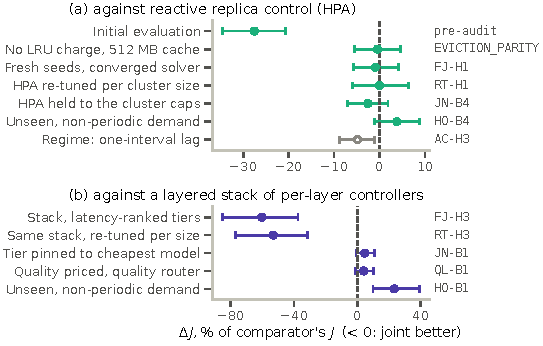
\includegraphics[width=\textwidth]{figures/fig_chain.pdf}
\caption{The joint controller's advantage disappears as its comparators
are corrected: \jcac{} minus comparator on $J$, per design point, as a
percentage of the comparator's $J$, with 95\% bootstrap intervals (negative:
\jcac{} better); each row keeps the corrections above it. The first two rows
of (a) are exploratory and did not share seeds; QL-B1 compares $J$ with
answer quality priced; the hollow row is a regime (replicas one interval
late), not a correction. The JN-B1 and HO-B1 stacks exceeded the cluster
caps; held to them, an exploratory re-run gives $-1.3\%$ and $+6.5\%$.}
\label{fig:chain}
\end{figure}

\emph{Against reactive replica control} (Fig.~\ref{fig:chain}(a)). The
pre-audit matrix put \jcac{} 27.5\% of HPA's $J$ ahead. Two comparator
defects produced that lead: only the comparators paid a $1.4581\times$
surcharge on inference cost (a model of LRU eviction that \jcac{}'s
cost-aware cache was assumed to avoid), and they ran a cache pinned at
128\,MB. Removing both erased it (EVICTION\_PARITY, $-0.4\%$). On fresh
shared seeds with the convergent solver the difference was $-0.0037$
$[-0.0234,+0.0166]$, a failed superiority test (FJ-H1). HPA's tuned target
lay on the edge of its grid; re-tuned per cluster size with an interior
optimum it tied again, $-0.0001$ $[-0.0239,+0.0257]$ (RT-H1), but the tie
hid a trade: \jcac{} spent 19.3\% less at 60.1\% higher mean violation, and
every SLO guard of that campaign failed. Held to the cluster caps that bind
\jcac{}, HPA still tied ($-0.0104$ $[-0.0290,+0.0076]$, JN-B4). \jcac{} beat
KEDA at its first fair setting ($-0.0305$, FJ-H2), tied it re-tuned
($-0.0309$ $[-0.0611,+0.0008]$, RT-H2) and beat it capped ($-0.0229$
$[-0.0438,-0.0022]$, JN-B5), a verdict that does not survive the
programme-wide correction.

\emph{Against a layered stack} (Fig.~\ref{fig:chain}(b)). The registered
layered stack lost by 60.4\% of its $J$ and, re-tuned per size, by 53.1\%
(FJ-H3, RT-H3), because its tier rule ranks tiers by latency and ignores
price: it reached the lowest violation of any arm at 3.4 times \jcac{}'s
spend (Table~\ref{tab:arms}). Pinned to the cheapest model, the same stack
tied \jcac{} ($+0.0178$ $[-0.0032,+0.0416]$, JN-B1), although it ran above
the cluster caps that bind \jcac{}; held to them, it still tied ($-0.0053$
$[-0.0201,+0.0092]$, exploratory). A cost-aware tier rule
lost by 0.3208 (JN-B2), and a quality-aware router tied when answer quality was priced (QL-B1).
The 53--60\% win measured one comparator's tier rule, not the value of
joint control.

Every defect we found in this chain had favoured the joint controller.
The corrections were applied one registered campaign at a time, and each
earlier record stands unedited beside its successor.

\subsection{What coordination is worth}
\label{sec:coordination}

\begin{table}[t]
\caption{Coordination in every registered setting where joint and
decoupled search ran on the same units: $\Delta J$ = joint minus decoupled
(negative: joint better), 95\% bootstrap CI, and the gain as a percentage
of the decoupled arm's $J$. EQ: CI inside $\pm0.025$. The width rows score
the 48 AI-carrying design points on the rate-limited lattice.}
\label{tab:coord}
\centering\footnotesize\setlength{\tabcolsep}{2.5pt}
\begin{tabular}{@{}l l r c r l@{}}
\toprule
Setting & Test & $\Delta J$ & 95\% CI & Gain & Reading \\
\midrule
Main matrix & JN-C1 & $-0.0066$ & $[-0.0121,-0.0022]$ & $+1.6\%$ & PASS, EQ \\
Cache curve fitted to LMSYS & CS-EQ & $-0.0064$ & $[-0.0110,-0.0029]$ & $+1.4\%$ & EQ \\
Published cache curve (rerun) & CS-EQ & $-0.0053$ & $[-0.0102,-0.0015]$ & $+1.3\%$ & EQ \\
High cache curve & CS-EQ & $-0.0042$ & $[-0.0085,-0.0009]$ & $+1.1\%$ & EQ \\
Answer quality priced ($J_q$) & QL-C1 & $+0.0012$ & $[-0.0016,+0.0043]$ & $-0.3\%$ & tie, EQ \\
Real BurstGPT windows & TA-EQ & $-0.0025$ & $[-0.0037,-0.0013]$ & $+0.6\%$ & EQ \\
Unseen, non-periodic demand & HO-C1 & $+0.0045$ & $[+0.0020,+0.0073]$ & $-1.4\%$ & worse, EQ \\
Live-fitted plant & RV-L-EQ & $-0.0017$ & $[-0.0028,-0.0008]$ & $+1.3\%$ & EQ \\
Width: published plant & WD-H4 & $-0.0044$ & $[-0.0088,-0.0006]$ & $+0.7\%$ & EQ \\
Width: coupled plant & WD-H4 & $-0.0092$ & $[-0.0181,-0.0019]$ & $+0.9\%$ & EQ \\
Width: live-fitted plant & WD-H4 & $-0.0033$ & $[-0.0048,-0.0019]$ & $+1.3\%$ & EQ \\
\bottomrule
\end{tabular}
\end{table}

With objective, forecast, budget filter, caps and lattice held fixed,
joint search lowered $J$ by $0.0066$ $[0.0022,0.0121]$ relative to
decoupled search, 1.6\% of the decoupled arm's $J$, and by $0.0009$
relative to knob-wise search (JN-C1, JN-C2; Table~\ref{tab:coord}). Both
reductions passed their directional tests (JN-C1 survives the
programme-wide Benjamini--Yekutieli correction but not Holm), and both lie
inside the equivalence margin. The decoupled arm spent 1.5\% less and violated
slightly more; coordination bought a little attainment, not savings.

Three qualifications bound this reading. First, the average is diluted: on
the 24 CRUD-only design points the two searches scored identically, as they
must when only the replica knob acts. On the 36 AI-carrying points the gain
was $0.0109$ $[0.0039,0.0198]$, and on the 12 small-cluster AI points
$0.0282$ $[0.0109,0.0503]$ (exploratory), an interval that reaches past the
margin. Second, the margin of $\pm0.025$ was set from the detectable
difference of the comparator contrasts; the joint--decoupled contrast is
far less noisy (its own detectable difference is about $0.007$), so
``inside the margin'' is a weak statement for it, and the interval itself,
0.5--3.0\% of $J$ overall, is the informative reading. Third, the
directional part rests on an unmeasured constant: with a monotone agent
latency ladder (small 0.94\,s, mid 2.5\,s, large 3.5\,s) and nothing else
changed, an exploratory re-run of one replication found no coordination
gain at all ($+0.0017$ $[-0.0020,+0.0061]$).

The result does not hinge on the synthetic cache curve or on the
objective. Under the cache curve fitted to real LMSYS prompts and under a
high one, $0.95\,c/(c+128)$, the reduction was 1.4\% and 1.1\% of $J$
(CS). With twice the answer-quality loss of Table~\ref{tab:tiers} added to
$J$, measured GPU prices and no budget filter, the difference was
$+0.0012$ (QL-C1), and on unseen demand decoupled search was the better of
the two, inside the margin (HO-C1). In all eleven registered settings the
difference stayed inside the registered margin.

\subsection{The complete policy after the corrections}
\label{sec:remains}

\begin{table}[t]
\caption{Mean outcome per arm in JOINTNESS (60 design points $\times$ 5
replications, shared seeds). Cost: simulated dollars per run. Viol.: mean
SLO violation. Excess: uncapped overshoot. Shed: tenant-steps with AI on
tier ``none''. Over.: tenant-steps over the tenant's budget (\jcac{} filters
on projected, not realised, cost).}
\label{tab:arms}
\centering\tablefont
% generated by make_assets.py -- do not edit
\begin{tabular}{@{}l r r r r r r@{}}
\toprule
Arm & $J$ & Cost & Viol. & Excess & Shed & Over. \\
 & & (\$) & & & (\%) & (\%) \\
\midrule
\jcac{}, joint search & 0.3991 & 2.36 & 0.068 & 0.207 & 7.2 & 0.9 \\
\jcac{}, decoupled search & 0.4057 & 2.33 & 0.072 & 0.209 & 7.7 & 0.8 \\
\jcac{}, knob-wise search & 0.4000 & 2.36 & 0.068 & 0.207 & 7.3 & 0.8 \\
\jcac{}, plans on violation & 0.4038 & 2.06 & 0.084 & 0.465 & 12.5 & 0.9 \\
\jcac{}, never sheds & 0.4668 & 2.81 & 0.075 & 0.533 & 0.0 & 4.5 \\
\midrule
Layered, cheapest tier & 0.3814 & 2.70 & 0.045 & 0.130 & 0.0 & 3.1 \\
Layered, cost-aware tier & 0.7199 & 4.35 & 0.113 & 0.630 & 0.0 & 7.3 \\
Layered, registered rule & 0.8631 & 7.97 & 0.012 & 0.029 & 0.0 & 10.4 \\
\midrule
Static equal share & 0.4226 & 2.91 & 0.052 & 0.177 & 0.0 & 3.5 \\
HPA, re-tuned & 0.4006 & 2.92 & 0.043 & 0.104 & 0.0 & 3.8 \\
HPA, re-tuned, capped & 0.4095 & 2.77 & 0.053 & 0.187 & 0.0 & 3.6 \\
KEDA, re-tuned, capped & 0.4220 & 2.93 & 0.051 & 0.172 & 0.0 & 3.8 \\
\bottomrule
\end{tabular}

\end{table}

\begin{table}[t]
\caption{What survives the corrections: \jcac{} minus comparator on $J$
(mean paired difference over design points, 95\% bootstrap CI; negative:
\jcac{} better). B: better; T: tie; W: worse; EQ: inside the $\pm0.025$
margin. The cheapest-tier stack was not held to the cluster caps (see
Section~\ref{sec:comparators}).}
\label{tab:post}
\centering\tablefont
% generated by make_assets.py -- do not edit
\begin{tabular}{@{}l l r c l@{}}
\toprule
Comparator & Test & $\Delta J$ & 95\% CI & \\
\midrule
\multicolumn{5}{@{}l}{\textit{Instant actuation} (60 design points)} \\
\quad Decoupled search & \texttt{JN-C1} & $-0.0066$ & $[-0.0121,-0.0022]$ & B, EQ \\
\quad Layered, cheapest tier & \texttt{JN-B1} & $+0.0178$ & $[-0.0032,+0.0416]$ & T \\
\quad Static equal share & \texttt{JN-B3} & $-0.0235$ & $[-0.0422,-0.0050]$ & B \\
\quad HPA, re-tuned, capped & \texttt{JN-B4} & $-0.0104$ & $[-0.0290,+0.0076]$ & T \\
\quad KEDA, re-tuned, capped & \texttt{JN-B5} & $-0.0229$ & $[-0.0438,-0.0022]$ & B \\
\midrule
\multicolumn{5}{@{}l}{\textit{Replicas one interval late} (60 design points)} \\
\quad Layered, cheapest tier & \texttt{AC-H1} & $+0.0069$ & $[-0.0135,+0.0300]$ & T \\
\quad Static equal share & \texttt{AC-H2} & $-0.0227$ & $[-0.0416,-0.0040]$ & B \\
\quad HPA, re-tuned, capped & \texttt{AC-H3} & $-0.0204$ & $[-0.0371,-0.0045]$ & B \\
\quad KEDA, re-tuned, capped & \texttt{AC-H4} & $-0.0279$ & $[-0.0474,-0.0089]$ & B \\
\midrule
\multicolumn{5}{@{}l}{\textit{Unseen, non-periodic demand} (24 design points)} \\
\quad Decoupled search & \texttt{HO-C1} & $+0.0045$ & $[+0.0020,+0.0073]$ & W, EQ \\
\quad Layered, cheapest tier & \texttt{HO-B1} & $+0.0629$ & $[+0.0268,+0.1065]$ & W \\
\quad Static equal share & \texttt{HO-B3} & $-0.0109$ & $[-0.0323,+0.0112]$ & T \\
\quad HPA, re-tuned, capped & \texttt{HO-B4} & $+0.0122$ & $[-0.0035,+0.0284]$ & T \\
\quad KEDA, re-tuned, capped & \texttt{HO-B5} & $-0.0151$ & $[-0.0377,+0.0073]$ & T \\
\bottomrule
\end{tabular}

\end{table}

\begin{figure}[t]
\centering
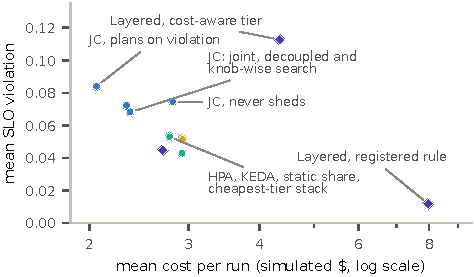
\includegraphics[width=0.62\textwidth]{figures/fig_tradeoff.pdf}
\caption{\jcac{} is the cheapest arm and among the most violating: mean
cost against mean SLO violation for every arm of Table~\ref{tab:arms}
(JOINTNESS). HPA, KEDA, the static share and the cheapest-tier stack
cluster at lower violation and 14--24\% higher cost; the never-shedding
variant of \jcac{} loses its cost advantage.}
\label{fig:tradeoff}
\end{figure}

With the defects removed, the complete-policy comparison is close
(Tables~\ref{tab:arms} and~\ref{tab:post}). \jcac{} tied capped HPA and the
cheapest-tier stack, and beat capped KEDA and the static share by
$0.0229$ and $0.0235$ in $J$, about 5.5\% (JN-B5, JN-B3). Its SLO guard
failed against all four: \jcac{}'s mean violation was 0.068, against
0.043--0.053 for every HPA, KEDA, static and cheapest-tier arm, which cost
14--24\% more (Fig.~\ref{fig:tradeoff}). Neither of the two wins survives
the programme-wide Holm correction.

\begin{figure}[t]
\centering
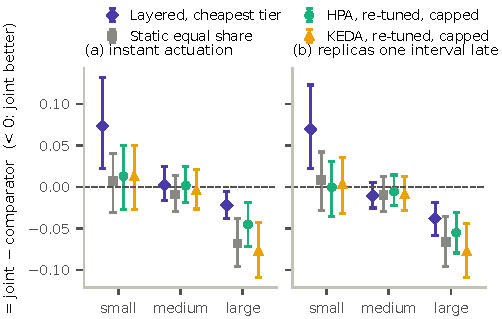
\includegraphics[width=0.62\textwidth]{figures/fig_sizes.pdf}
\caption{Every win of \jcac{} comes from the large cluster: \jcac{} minus
comparator on $J$ per cluster size, 20 design points each, 95\% bootstrap
intervals, (a) with instant actuation (JOINTNESS) and (b) with replicas
one interval late (ACTUATION). On the small cluster the cheapest-tier stack
is better in both regimes, but it ran twice that cluster's replica cap; held
to the caps it ties (exploratory, not plotted).}
\label{fig:sizes}
\end{figure}

The wins are not spread across the matrix (Fig.~\ref{fig:sizes}).
\jcac{} beat every comparator on the large cluster, by $0.0220$ to $0.0771$
in $J$ against the four competitive ones; it tied every one on the medium
cluster; and on the small cluster the cheapest-tier stack beat it by
$0.0732$ $[0.0227,0.1314]$, but that stack ran twice the small cluster's
replica cap there, and held to the caps it tied \jcac{} ($+0.0066$,
exploratory). By workload,
the wins came with the CRUD classes, where only the replica knob acts and
\jcac{} was better than every comparator but the cost-aware stack on all 12
steady-CRUD design points: on the 24 CRUD points it beat capped KEDA and the
static share by about 0.05 in $J$, which is replica sizing against
comparators whose single tuned target over-provisions CRUD
(Section~\ref{sec:comparators}). On the 36 design points that carry AI
traffic, where the cache and tier knobs act, \jcac{} tied capped HPA
($-0.0043$ $[-0.0341,+0.0245]$), capped KEDA ($-0.0053$) and the static
share ($-0.0056$), and lost to the uncapped cheapest-tier stack ($+0.0446$
$[+0.0124,+0.0809]$); on the agentic class it was worse than every
comparator except the cost-aware stack. Nor did it use its tier knob much:
it chose the large tier on no tenant-step and the mid tier on 1.7\%, so in
practice its tier decision was ``small or shed''. The controller built to
coordinate the AI knobs gained nothing on the workloads those knobs serve.

\subsection{Where the savings come from: shedding}
\label{sec:shed}

\begin{table}[t]
\caption{Total cost and cost per request actually served. Shed: share of
requests answered by no model. Unit: the ratio averaged over design points
(main matrix) or windows (BurstGPT); pooled: taken over all requests of all
runs (exploratory). Counts come from request counters added to the
simulator without changing any registered metric (SA: 27{,}720 registered
values replayed bit-identically).}
\label{tab:served}
\centering\footnotesize\setlength{\tabcolsep}{2.5pt}
\begin{tabular}{@{}l r r r r r@{}}
\toprule
 & Cost & Shed (\%) & Shed (\%) & \$/1{,}000 served & \$/1{,}000 served \\
Arm & (\$/run) & unit & pooled & unit & pooled \\
\midrule
\multicolumn{6}{@{}l}{\textit{Main matrix (JN runs, 180{,}773 requests per run)}} \\
\quad \jcac{}, joint search & 2.363 & 5.7 & 2.1 & 0.0340 & 0.01335 \\
\quad \jcac{}, decoupled search & 2.328 & 6.0 & 2.2 & 0.0336 & 0.01317 \\
\quad \jcac{}, never sheds & 2.809 & 0.0 & 0.0 & 0.0367 & 0.01554 \\
\quad HPA, re-tuned, capped & 2.775 & 0.0 & 0.0 & 0.0338 & 0.01535 \\
\quad KEDA, re-tuned, capped & 2.926 & 0.0 & 0.0 & 0.0349 & 0.01619 \\
\quad Layered, cheapest tier & 2.698 & 0.0 & 0.0 & 0.0331 & 0.01493 \\
\quad Static equal share & 2.910 & 0.0 & 0.0 & 0.0348 & 0.01610 \\
\midrule
\multicolumn{6}{@{}l}{\textit{Real BurstGPT windows (TA runs, 804{,}710 requests per run)}} \\
\quad \jcac{}, joint search & 34.70 & 14.7 & 42.8 & 0.4687 & 0.07545 \\
\quad \jcac{}, decoupled search & 34.24 & 15.0 & 43.4 & 0.4689 & 0.07523 \\
\quad \jcac{}, never sheds & 79.00 & 0.0 & 0.0 & 0.4783 & 0.09817 \\
\quad HPA, re-tuned, capped & 69.52 & 0.0 & 0.0 & 0.2950 & 0.08640 \\
\quad KEDA, re-tuned, capped & 69.94 & 0.0 & 0.0 & 0.3001 & 0.08691 \\
\quad Layered, cheapest tier & 68.06 & 0.0 & 0.0 & 0.2890 & 0.08457 \\
\quad Static equal share & 76.17 & 0.0 & 0.0 & 1.2468 & 0.09465 \\
\bottomrule
\end{tabular}
\end{table}

\jcac{} shed AI traffic on 7.2\% of tenant-steps. Request counters, added to
the simulator as a registered re-run that left every registered metric
bit-identical (SA), show what that means: on the mean design point it left
10.1\% of AI requests (5.7\% of all requests) unanswered by any model, and
35.3\% of the agentic class's AI requests (Table~\ref{tab:served}). On the
BurstGPT windows it left 14.7\% unserved on the mean window and 42.8\% of
all requests pooled, because it sheds when demand, and so spend, peaks. The
decoupled and knob-wise arms shed as often (7.7\% and 7.3\% of
tenant-steps), so the savings come from shedding, not from coordination.

Shedding is where the cost advantage lives. Forbidden to shed, \jcac{} cost
19\% more than with shedding, slightly more than capped HPA; its $J$ rose by
$0.0677$ $[0.0432,0.0945]$, and it lost to capped HPA by $0.0573$
$[0.0225,0.0938]$ (JOINTNESS) and, on the BurstGPT windows, by $0.2229$.
That registered variant is handicapped, however: when no affordable
candidate exists, its fallback cuts two replicas and a cache level while
still serving over budget, so it misses more and pays more. With a fallback
that holds its configuration instead, an exploratory re-run of the AI
design points (one replication) improved its $J$ by 0.096 at 2.7\% lower
cost, which would put it close to capped HPA overall. The cost increase of
forbidding shedding (16--19\%) survives that correction; the loss to capped
HPA may not.

Billing each shed request at the cheapest tier's price, as if it had been
served there, removes every dollar advantage \jcac{} has and, in $J$, turns
the tie with capped HPA into a loss ($+0.0295$ $[0.0045,0.0562]$) and the
wins over capped KEDA and the static share into ties (exploratory
re-scoring of the registered runs). Per AI request actually served,
\jcac{} paid the most of the main arms (\$0.110 per 1{,}000 against
\$0.103 for the cheapest-tier stack and \$0.106 for capped HPA; 7--9\% more
on the small cluster), because it holds less cache and buys the mid tier for
some agent traffic (exploratory, one replication). Over all requests,
whether \jcac{} is cheaper per request served depends on how the ratio is
aggregated (Table~\ref{tab:served}): per design point or window it is not
(dearer than the cheapest-tier stack by 2.7\% on the matrix and 62\% on the
BurstGPT windows); pooled over requests it is about 11\% cheaper, because
cheap CRUD requests dominate the pool and it drops the most traffic where
traffic is heaviest. We claim no per-request saving.

Not every shed is the objective's choice (exploratory analysis of one
replication; the registered SA record counts sheds but not their cause). Of
\jcac{}'s shed decisions on
the AI design points, 58\% were forced: no candidate fit the budget. The
other 42\% were voluntary (an affordable candidate existed), including every
shed of a premium tenant. The budgets themselves set the scale of the
forced part: on the BurstGPT windows a \$5 hourly budget pays for at most
about 19 chat requests per second even on the small tier with a full cache,
while heavy windows average 11--17 and peak at 50 per tenant, so much of the
42.8\% pooled shed reflects the budgets we chose, not only the controller.

$J$ is what makes this pay. As derived in Section~\ref{sec:objective}, $J$
values an AI outage at no more than $2q_{\mathrm{AI}}$ per tenant-step,
less than the model spend of many intervals. Adding $\kappa s$ to $J$, with
$s$ the share of tenant-steps an arm sheds, erases \jcac{}'s wins over
capped KEDA and the static share at $\kappa\approx0.32$ (95\% intervals
within $[0.02,0.79]$) and its point advantage over capped HPA at
$\kappa\approx0.14$ (exploratory, RV); for scale, \jcac{}'s $J$ is 0.40. On the
live-fitted plant, where no comparator ever violated an SLO, \jcac{} still
shed on 14.2\% of tenant-steps, cost more than the cheapest-tier stack
(\$1.16 against \$1.02 per run) and lost to it by $0.0268$ in $J$ (RV-L3):
there, the (uncapped) stack serving every request on the cheapest model
dominated the joint controller on cost, violation and fairness at once.

\subsection{Budgets and actuation lag}
\label{sec:budget}

Only \jcac{} filters its candidates by the tenant's budget, which can only
hurt it on $J$ (which ignores budgets), so BM re-ran the comparators under
the same filter. Capped HPA and KEDA then lost to \jcac{} by $0.0316$
$[0.0154,0.0495]$ and $0.0416$ $[0.0242,0.0598]$ on the main matrix
(BM-H1, BM-H2) and by about 0.17 on the BurstGPT windows; the
budget-filtered cheapest-tier stack still tied ($-0.0011$
$[-0.0221,+0.0212]$, BM-H3). These wins must be read for what the filter
did. Because the comparators' cache and tier rules stayed their own, the
filter could only trim replicas; it lowered their spend by about 1\% and
left them over budget on 2.2--3.2\% of tenant-steps, while raising their
violation by about 0.009 (on the windows, from 0.017 to 0.074). BM therefore
shows that trimming replicas to meet a budget does not work when model
spend dominates, as an earlier campaign had predicted
(BUDGET\_PARITY), not that \jcac{} beats a budget-compliant autoscaler.
No budget-compliant comparator that serves every request exists in this
plant; the fair comparator, a per-layer stack whose gateway refuses AI
calls once a tenant's budget is spent, is the gated stack of the final
campaign (Section~\ref{sec:level}).

Actuation lag is the one regime in which \jcac{} beat the reactive rules
with its SLO guard intact. With replica changes taking effect one interval
late and enlarged caches half-warm, \jcac{} beat capped HPA by 4.8\%
($-0.0204$ $[-0.0371,-0.0045]$, AC-H3) and capped KEDA by 6.5\%
($-0.0279$, AC-H4), and both guards passed: a planner with a horizon
anticipates what a reactive rule can only follow. It still tied the
cheapest-tier stack (AC-H1), tier switches never lagged, and the plant had
no request backlog. Both verdicts survive the programme-wide
Benjamini--Yekutieli correction but not Holm.

\subsection{Generalisation}
\label{sec:generalise}

Every positive result above was obtained on the periodic workloads that
the comparators were tuned on. On two held-out Markov-modulated workloads,
registered before any arm ran on them, \jcac{} beat no comparator, and the
cheapest-tier stack beat it by $0.0629$ $[0.0268,0.1065]$, 23.3\% of the
stack's $J$, on every cluster size, the large one included (HO-B1;
Table~\ref{tab:post}, last block). Every SLO guard failed: the stack held
violation at 0.004 against \jcac{}'s 0.056, while \jcac{} shed on 11.3\% of
tenant-steps. Part of that margin was the stack's excess hardware: held to
the cluster caps (exploratory), it still beat \jcac{}, by $0.0202$
$[0.0039,0.0361]$ or 6.5\% of its $J$.

On the 96 real BurstGPT windows, \jcac{} beat only the static share
($-0.0913$ $[-0.1751,-0.0290]$, TA-H4), at an SLO excess of 0.34 against
0.02. It did not beat capped HPA ($-0.0530$ $[-0.1376,+0.0095]$, better in
31\% of windows), capped KEDA, or the uncapped cheapest-tier stack
($-0.0132$ $[-0.0611,+0.0239]$, better in 23\% of windows). On a plant re-fitted to
the deployed gateway's measurements, a planner that kept believing the
published plant lost to the registered layered stack by $0.1052$
(SM-H2[live]), and \jcac{} planning on the fitted plant trailed the
uncapped cheapest-tier stack by $0.0268$ (RV-L3). None of the joint controller's
advantages over a tuned, cheapest-model per-layer stack holds outside the
setting it was designed in.

\subsection{At a level field: the final campaign}
\label{sec:level}

\begin{table}[t]
\caption{LEVEL, the final campaign (8{,}832 runs, all valid, fresh seeds):
the corrected joint controller minus each comparator on $J_L$ (the objective
with every refused request charged the small tier's price), mean paired
difference over design points or windows and 95\% bootstrap CI (negative:
\jcac{} better). One Holm family of eleven; below the rule, coordination
(joint minus decoupled search) against the registered $\pm0.01$ margin.}
\label{tab:level}
\centering\scriptsize\setlength{\tabcolsep}{2.5pt}
% generated by make_tables.py -- do not edit
\begin{tabular}{@{}l l l r c l@{}}
\toprule
Test & Substrate & Comparator & $\Delta J_L$ & 95\% CI & Verdict \\
\midrule
\texttt{LV-B1} & main & Cheapest-tier stack, budget-gated & $+0.0038$ & $[-0.0130,+0.0207]$ & FAIL \\
\texttt{LV-B2} & main & HPA, capped & $+0.0208$ & $[-0.0026,+0.0441]$ & FAIL \\
\texttt{LV-B3} & main & KEDA, capped & $+0.0088$ & $[-0.0174,+0.0350]$ & FAIL \\
\texttt{LV-B4} & main & Cheapest-tier stack, capped & $+0.0282$ & $[+0.0070,+0.0496]$ & FAIL \\
\texttt{LV-B5} & main & Static equal share & $+0.0081$ & $[-0.0164,+0.0324]$ & FAIL \\
\texttt{LV-P1} & main & JC, published & $-0.0095$ & $[-0.0234,+0.0040]$ & FAIL \\
\texttt{LV-R1} & mono & Cheapest-tier stack, budget-gated & $+0.0046$ & $[-0.0121,+0.0207]$ & FAIL \\
\texttt{LV-L1} & lag & Cheapest-tier stack, budget-gated & $+0.0335$ & $[+0.0108,+0.0560]$ & FAIL \\
\texttt{LV-L2} & lag & HPA, capped & $+0.0518$ & $[+0.0245,+0.0789]$ & FAIL \\
\texttt{LV-O1} & held-out & Cheapest-tier stack, budget-gated & $+0.1230$ & $[+0.0982,+0.1484]$ & FAIL \\
\texttt{LV-T1} & BurstGPT & Cheapest-tier stack, budget-gated & $-0.0152$ & $[-0.0186,-0.0118]$ & PASS \\
\midrule
\texttt{LV-C[LV]} & main & decoupled search & $-0.0119$ & $[-0.0173,-0.0071]$ & not EQ at $\pm0.01$ \\
\texttt{LV-C[MO]} & mono & decoupled search & $-0.0120$ & $[-0.0181,-0.0065]$ & not EQ at $\pm0.01$ \\
\texttt{LV-C[LG]} & lag & decoupled search & $-0.0095$ & $[-0.0143,-0.0053]$ & not EQ at $\pm0.01$ \\
\texttt{LV-C[HO]} & held-out & decoupled search & $-0.0212$ & $[-0.0300,-0.0127]$ & not EQ at $\pm0.01$ \\
\texttt{LV-C[TR]} & BurstGPT & decoupled search & $-0.0070$ & $[-0.0097,-0.0046]$ & EQ at $\pm0.01$ \\
\bottomrule
\end{tabular}

\end{table}

\begin{table}[t]
\caption{Mean outcome per arm in LEVEL's main matrix (60 design points
$\times$ 5 replications). Shed: share of requests refused; Over.:
tenant-steps over budget. Every arm obeys the cluster caps.}
\label{tab:levelarms}
\centering\footnotesize\setlength{\tabcolsep}{4pt}
% generated by make_tables.py -- do not edit
\begin{tabular}{@{}l r r r r r r@{}}
\toprule
Arm & $J_L$ & $J$ & Cost & Viol. & Shed & Over. \\
 & & & (\$) & & (\%) & (\%) \\
\midrule
JC, level (treatment) & 0.4278 & 0.4076 & 2.31 & 0.074 & 3.2 & 0.7 \\
JC, level, decoupled search & 0.4398 & 0.4148 & 2.28 & 0.079 & 3.9 & 0.7 \\
JC, published & 0.4374 & 0.3972 & 2.35 & 0.068 & 5.8 & 0.8 \\
\midrule
Cheapest-tier stack, budget-gated & 0.4240 & 0.4069 & 2.51 & 0.066 & 2.3 & 0.7 \\
Cheapest-tier stack, capped & 0.3997 & 0.3997 & 2.67 & 0.054 & 0.0 & 3.3 \\
HPA, capped & 0.4070 & 0.4070 & 2.77 & 0.053 & 0.0 & 3.6 \\
KEDA, capped & 0.4191 & 0.4191 & 2.93 & 0.051 & 0.0 & 3.8 \\
Static equal share & 0.4197 & 0.4197 & 2.91 & 0.052 & 0.0 & 3.6 \\
\bottomrule
\end{tabular}

\end{table}

The twelfth campaign removed the audited leaks on both sides at once
(Section~\ref{sec:levelmethod}) and asked RQ1 and RQ2 again on fresh seeds.
All 8{,}832 runs were valid; of eleven registered tests, one passed
(Table~\ref{tab:level}). We had predicted three passes, and all three failed;
the one test that passed was predicted to fail.

On the main matrix the corrected controller beat no comparator. It tied the
budget-gated stack ($+0.0038$ $[-0.0130,+0.0207]$), capped HPA, capped KEDA
and the static share, and the capped cheapest-tier stack without a gate was
better than it ($+0.0282$ $[+0.0070,+0.0496]$; Table~\ref{tab:levelarms}). The
fixes did not make it better than the published controller under $J_L$
($-0.0095$ $[-0.0234,+0.0040]$): pricing the outage cut its refused share from
5.8\% to 3.2\% of requests, but its violation rose from 0.068 to 0.074. The
monotone agent row changed nothing (LV-R1). Under one-interval actuation lag
the corrected controller lost to the gated stack ($+0.0335$) and to capped HPA
($+0.0518$), the reverse of ACTUATION. The arms explain why: under lag its $J_L$
rose by 0.043, the published controller's by 0.001. The published switching
penalty ratchets replicas upward (Section~\ref{sec:objective}); under instant
actuation that is a defect, but under lag it is a hedge, and the corrected
penalty, which lets replicas fall and rise again, pays for every replica that
arrives late. The variant was chosen under instant actuation, where that cost
is invisible. On the held-out workloads the gated stack beat it by $0.1230$
$[0.0982,0.1484]$.

The one registered win came on the real BurstGPT windows, where the budgets
bind hardest. Among the arms that keep the budget, the corrected controller
beat the budget-gated stack by $0.0152$ $[0.0118,0.0186]$, 2.7\% of the stack's
$J_L$, in 91\% of windows, at 13\% lower cost and the same refused share (14.4\%
of requests): budget-aware joint planning beat a reactive gate there. The
comparators that ignore the budget (capped HPA, capped KEDA and the ungated
stack), which spent more than twice as much and served every request, scored
better than both ($J_L$ 0.439--0.441 against 0.552). Which of the two is
preferable depends on whether a budget is a hard constraint; $J_L$ treats it
as a soft one.

Coordination grew once outages were priced (Table~\ref{tab:level}, lower
block): joint search beat decoupled search by 1.3--4.5\% of $J_L$, with every
interval below zero. Only on the BurstGPT windows did the difference fall
inside the registered $\pm0.01$ margin, and on the held-out workloads (4.5\%) it
exceeded even $\pm0.025$. The mechanism of Section~\ref{sec:width} bounds
coordination; it does not make it zero. When a refused request costs money,
the planner has more to trade between cache and tier, and the gain grows by
about two-thirds over JOINTNESS. It still bought no win against a level
per-layer stack.

\subsection{Why coordination buys little}
\label{sec:width}

For a move $\delta=(\delta_r,\delta_c,\delta_\tau)$ of one tenant, the
second-order change in $\Phi$ is
$\sum_k g_k\delta_k+\frac12\sum_{k,l}H_{kl}\delta_k\delta_l$. Decoupled
search sees every term except the cross terms ($k\neq l$), so it recovers the
joint move unless a cross term reverses a per-knob choice. First-order gains
grow with $|\delta|$ and cross terms with $|\delta|^2$, so small steps make
reversals rare. Near a resting optimum the gradient vanishes and
separability needs small cross terms instead, which is what Bristol's
relative gain array tests~\cite{bristol1966}. In this plant, cache and tier
always interact through the price of a miss, and the replica knob interacts
with the others only where AI work loads the replicas. The argument is a
heuristic (the tier is categorical), but it makes two predictions:
coordination should grow with the step size, and only on plants where the
layers share capacity.

\begin{figure}[t]
\centering
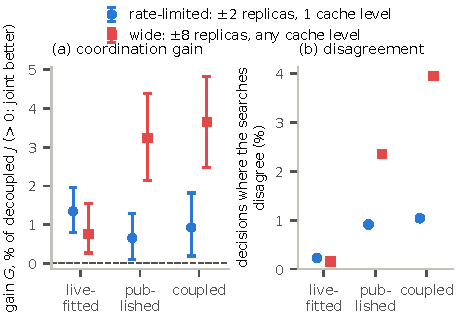
\includegraphics[width=0.62\textwidth]{figures/fig_width.pdf}
\caption{Coordination grows with step width, and only on plants where AI
work loads the replicas. (a) Gain $G=J(\text{decoupled})-J(\text{joint})$
as a percentage of the decoupled arm's $J$, with 95\% bootstrap intervals.
(b) Share of best responses in which decoupled search would choose
differently. 48 AI-carrying design points $\times$ 5 replications per
plant.}
\label{fig:width}
\end{figure}

\begin{table}[t]
\caption{The width experiment: coordination gain $G$ on the rate-limited
($n$) and wide ($w$) lattices, their difference-in-differences (DiD), and
the joint controller's own $J$ on the rate-limited minus the wide lattice
(negative: rate-limited better).}
\label{tab:width}
\centering\tablefont
% generated by make_assets.py -- do not edit
\begin{tabular}{@{}lrrcr@{}}
\toprule
Plant & $G_n$ & $G_w$ & DiD [95\% CI] & $J_n-J_w$ \\
\midrule
Live-fitted & $+0.0033$ & $+0.0021$ & $-0.0012$ $[-0.0032,+0.0009]$ & $-0.0301$ \\
Published & $+0.0044$ & $+0.0231$ & $+0.0187$ $[+0.0082,+0.0287]$ & $-0.0152$ \\
Coupled & $+0.0092$ & $+0.0407$ & $+0.0315$ $[+0.0161,+0.0472]$ & $-0.0859$ \\
\midrule
Tests & \multicolumn{2}{l}{\texttt{WD-H4}: EQ, all} & \texttt{WD-H1}, \texttt{H2} PASS; \texttt{H3} EQ & \texttt{WD-H5} PASS \\
\bottomrule
\end{tabular}

\end{table}

The WIDTH campaign tested both on three plants: the published one; the
coupled one, in which AI work loads the replicas three times as heavily;
and the live-fitted one, in which it never does. Joint and decoupled search
ran on the published lattice and on a wide one ($\Delta r\in\{-8,\dots,8\}$,
any cache level; up to 408 candidates per tenant instead of 60). All five
registered predictions held (Fig.~\ref{fig:width}, Table~\ref{tab:width}).
On the rate-limited lattice the gain was 0.7--1.3\% of the decoupled arm's
$J$ and equivalent to zero on every plant (WD-H4), and the searches chose
differently in at most 1.04\% of best responses. With wide steps the gain
rose by $0.0187$ $[0.0082,0.0287]$ on the published plant and $0.0315$
$[0.0161,0.0472]$ on the coupled one, 5.3 and 4.4 times its rate-limited
value (WD-H1, WD-H2), with disagreement of 2.4\% and 3.9\%; on the
live-fitted plant it did not rise ($-0.0012$ $[-0.0032,+0.0009]$, EQ,
WD-H3). Wide steps also made the joint controller itself worse on every
plant, by $0.0152$, $0.0859$ and $0.0301$ in $J$ on the published, coupled
and live-fitted plants (WD-H5): coordination pays only in a regime this
controller should avoid. WIDTH scores the 48 AI-carrying design points and
followed exploratory probes on disjoint seeds, so it is a confirmatory
replication of a pattern we had already seen, not a blind test; WD-H1 and
WD-H5 on the published plant passed in their families but not under the
programme-wide Holm correction.

\subsection{What ran on a real cluster}
\label{sec:live}

The control loop also ran live, but the live evidence is a case study and
supports none of the comparisons above. On one rented host with an L40S GPU
serving three Qwen2.5 models through vLLM, a registered four-cell
experiment (one run per arm and cell) found the published controller 23.3\%
dearer than its own tier-only ablation in the stress cell (WL-H1 FAIL): the
tier knob alone carried the gain. Two controller defects were diagnosed (an
open-loop plant model and a hysteresis ratchet) and a corrected,
calibrated controller was registered and run the same day on the same
cells, two replications each; it was 17.7\% cheaper than the tier-only arm
and 20.5\% cheaper than the published controller at equal fairness, with
intervals over autocorrelated 10\,s buckets. That evidence is weak by
construction: one host, two replications, a controller calibrated on the
cells it was scored on, a primary latency measurand that was not scraped
in the first sitting, and a replica-only comparator voided because a
preflight step left it on the large tier (the void comparison is not
quoted). A later registered damping variant failed both its predictions.
The live planner also under-read CRUD demand behind replicated pods (each
pod stamped its own rate), a defect found after these runs; its effect on
the verdicts was not measured. Separately, a 24-hour soak of the deployed
system served 25.8 million requests with none dropped and no pod restarts,
but failed its recovery and hourly-latency criteria. A registered five-seed
live replication of the corrected controller was designed and not funded.

% =====================================================================
\section{Lessons}
\label{sec:lessons}
% =====================================================================

\paragraph{When a joint controller is worth building}
For planners of this kind, joint search earns its cost only when one
interval may move a tenant far relative to its size \emph{and} the layers
share a resource. The rate-limited lattice moves a tenant by at most
one-eighth to one-third of its replica cap per interval; the wide lattice
by half or more. Kubernetes' default HPA scale-up policy, which may double
a deployment or add four pods every 15\,s~\cite{k8shpa}, resembles the wide
lattice at 6 to 16 replicas, so the regime in which coordination pays is
not exotic; but in our plant it was also the regime in which the planner
did worst. Whether a deployment is in the separable regime can be checked
before anything is built: probe the disagreement between joint and per-knob
best responses on recorded states, as Fig.~\ref{fig:width}(b) does, in the
spirit of Bristol's interaction measure~\cite{bristol1966}. Below a few
percent disagreement, three well-tuned loops will do.

\paragraph{What to build instead}
In this plant the bill is model spend, and the decision that moves it is
the tier. A per-layer stack with a tuned, capped autoscaler and the
cheapest adequate model matched the joint controller on the matrix and beat
it on unseen demand, also when held to the cluster caps, and on the
live-fitted plant. What the joint
controller added that the stack lacked was a hard per-tenant budget, which
it kept by refusing service. A budget is an operator policy and should be
enforced, and reported, as one: a gateway that refuses AI calls once a
tenant's budget is spent makes the trade explicit, whereas an objective that
prices the refusal through a capped violation term hides it. The final
campaign gave a per-layer stack exactly that gate. On the synthetic matrix
the gate rarely fired and the gated stack tied the joint controller; on real
BurstGPT demand, where the budgets bind, the joint controller kept them at a
lower cost than the gate did. That is the one place our evidence favours a
budget-aware planner over a reactive layer, and it is narrow: arms that
simply overspent the budget scored better still.

\paragraph{Fixes interact with the actuation model}
The published controller's switching penalty ratchets replicas upward, which
the audit flagged as a defect, and the corrected penalty was the treatment's
best variant on the instant-actuation tuning slice. Under one-interval lag
the ranking reversed: the ratchet held replicas the plant could not deliver
in time anyway, while the corrected controller paid for every replica that
arrived late, and it lost to the reactive stacks it had tied. Hysteresis in a
controller is a bet on the actuation model, and a variant selected under one
model needs a registered test under the others before it is called a fix.

\paragraph{How to evaluate a joint controller}
Every comparator defect we found favoured the joint controller.
Table~\ref{tab:checklist} turns them into rules, each paired with the
defect it caught here and the effect of correcting it. None of the rules is
new on its own~\cite{chameleon,hoefler2015}; what this study adds is a
measurement of how much each was worth in one realistic evaluation, and
the observation that they compound: the first two corrections alone
removed a 27.5\% lead, and the fourth removed a 60\% one.

\begin{table}[t]
\caption{Rules for comparing a joint controller with per-layer
controllers, the defect each caught in this study, and the effect of
correcting it on the joint controller's measured advantage ($\Delta J$ as
a percentage of the comparator's $J$; negative: joint better).}
\label{tab:checklist}
\centering\tablefont
\begin{tabular}{@{}>{\raggedright\arraybackslash}p{0.25\textwidth}
                >{\raggedright\arraybackslash}p{0.36\textwidth}
                >{\raggedright\arraybackslash}p{0.31\textwidth}@{}}
\toprule
Rule & Defect it caught & Effect (campaign) \\
\midrule
One cost model for all arms & Only baselines paid a $1.4581\times$
  inference surcharge; their cache was pinned at 128\,MB &
  $-27.5\%\rightarrow-0.4\%$ (EVICTION\_PARITY) \\
Interior tuning optima, per cluster size & HPA's optimum on a grid edge &
  $-0.9\%\rightarrow0.0\%$ (RT-H1) \\
Same caps, budgets and action set for all arms & Re-tuned HPA and the
  cheapest-tier stack ran up to twice the small cluster's replica cap; only
  the joint controller kept budgets or could shed &
  capped HPA still a tie (JN-B4); capped stack: small-cluster loss
  $+0.0732\rightarrow+0.0066$ (exploratory); with caps, a budget gate and an
  outage price for all, no joint win on the matrix (LEVEL) \\
A cheapest-adequate per-layer stack & Registered tier rule ranked tiers by
  latency, at 3.4$\times$ the cost & $-60.4\%\rightarrow+4.7\%$ (JN-B1) \\
A decoupled-search ablation & Coordination never isolated &
  1.6\% of $J$, inside the margin (JN-C1) \\
Count requests served; price outages & $J$ priced a shed request only
  through a capped violation term & 10.1\% of AI requests unserved; priced
  and level, no win on the matrix (SA, LEVEL) \\
Held-out demand & Every workload periodic, comparators tuned on them &
  $+23.3\%$ against the cheapest-tier stack (HO-B1); $+6.5\%$ with the stack
  capped (exploratory) \\
\bottomrule
\end{tabular}
\end{table}

\paragraph{For multi-loop self-adaptive systems}
The question of when separate adaptation loops need a coordinator is
usually argued from the loops' interactions~\cite{weyns2013,kephart2007}.
Our results suggest it can also be answered by measurement, and that the
answer depends on two properties an engineer controls: how far each loop
may move per decision, and whether the loops' effects meet in a shared
resource. Rate limits, which operators impose for stability anyway, make
the joint problem locally separable and the coordinator nearly redundant.
This is one plant and one family of planners; whether the regularity holds
for other multi-loop systems is an open, testable question.

% =====================================================================
\section{Threats to validity}
\label{sec:threats}
% =====================================================================

\paragraph{Construct validity}
The plant is our own model, and the planner plans with that same model:
it is an oracle of the system it controls, which flatters \jcac{} against
comparators that see only utilisation or request rates. On a plant
re-fitted to the deployed gateway's measurements, a planner that kept the
published model lost to the layered stack by $0.1052$ in $J$. The plant's
replicas are gateway pods, not GPU model servers: batching, KV-cache
memory, request backlog and tier-switch lag lie outside the study, and
pod congestion multiplies the external model's latency instead of adding a
queueing delay. A replica-step costs about one small-tier cache miss while
a tenant sends tens of misses per step, so the bill is mostly model spend,
set by a synthetic price ladder of 1:10:100 per miss in ten of the eleven
campaigns; our own GPU bench measured 1:1.475:1.518. Under the measured
ladder coordination was worth nothing (QUALITY), and the complete-policy
verdicts move: in an exploratory re-run of JOINTNESS under that ladder,
\jcac{} beat every comparator, the cheapest-tier stack by $0.0276$
$[0.0045,0.0531]$, but only because the comparators stayed pinned to the
small tier and because small-tier agent requests are slow by assumption.
That assumption (6\,s on the small tier against 2.5 and 3.5\,s on the
larger ones) is unmeasured and contradicted by our own bench; with a
monotone ladder the directional coordination gain disappeared and
\jcac{}'s wins over capped KEDA and the static share became ties
(exploratory). At the level field of LEVEL the monotone row changed no
verdict (LV-R1), so the final RQ1 answer does not rest on it; the
synthetic price ladder was not varied there and remains an assumption under
every final verdict. RQ2's conclusion that coordination is small holds under
both rows and both ladders. The cache is a synthetic hit
curve, bounded by the CS campaign but with no model of similarity,
eviction, drift or wrong answers; its memory is almost free (0.2\% of the
bill), so more cache is always better up to the caps. $J$ uses the planner's own
weights; it ignores budget overruns (3.1--10.4\% of the comparators'
tenant-steps), prices a shed request only through a capped violation term,
leaves network, storage and control-plane cost unpriced, and includes
answer quality only in QUALITY. In an exploratory re-scoring, the registered
violation weight of 2 was exactly the crossover against re-tuned HPA (at 4
HPA was better, at 8 KEDA too) and the re-scoring did not re-optimise the
arms at each weight. The cost per request served changes sign with its
aggregation (Section~\ref{sec:shed}), so we make no per-request cost claim.
The budgets were set below the small tier's peak spend for several
workloads, so part of the shedding is a property of the budgets we chose.

\paragraph{Internal validity}
The comparators are hand-written rules with one or two parameters, tuned
on a 12-run slice; per-size re-tuning moved their cost and violation but
barely their $J$, because $J$ is nearly flat in their targets. The
registered layered stacks were not held to the cluster caps, and the
cheapest-tier stack used up to twice the small cluster's replicas; its
capped re-run is exploratory and was not re-tuned under the caps. In the
first eleven campaigns only \jcac{} could shed or keep a budget, and the
budget-matched campaign could not remove that asymmetry
(Section~\ref{sec:budget}). LEVEL removed both leaks (every arm capped and
re-tuned; a budget-gated stack), but its own choices carry risk: the
treatment variant was selected on the comparators' tuning slice under
instant actuation, which is how a variant fragile under lag was chosen; the
gate sheds whole steps, as \jcac{} does, rather than refusing only the
requests beyond the budget; and the comparators were not re-tuned for lag,
held-out demand or the trace. \jcac{} plans one held move
per interval on a three-point trend forecast; a damped Holt forecaster cut
one-step error on the BurstGPT trace by 6.9--26.9\%, but joint and
decoupled search share the forecast, so RQ2 is unaffected. A multi-step
planner might find sequenced coordination that a held move cannot; the
wide-lattice \jcac{} beat neither the default-behaviour nor the capped HPA
(RV-W1, RV-W2). The solver is joint within a tenant and coordinate descent
across tenants; on the earlier, non-convergent solver, six sweep orders moved
mean Jain fairness by at most 0.0076 and cost by 0.91\%. Actuation is
instantaneous outside ACTUATION, and even there tier switches never lag.
Besides the comparator defects of Section~\ref{sec:chain}, our audits found
two defects that hurt \jcac{} (the non-convergent solver, replaced in every
campaign here, and the comparators' missing budget, which BM measures) and
several in the live harness (Section~\ref{sec:live}).

\paragraph{External validity}
The main workloads are synthetic and periodic, every design point puts
eight tenants of a single workload class together (so tenants interact
only through the cluster caps), HELDOUT has one AI class, the coupled plant was chosen from a probe grid, and the live-fitted
plant is a parameter scenario, not a live experiment: no measured run
reached congestion and AI requests never loaded a replica, so the coupling
that coordination needs was absent from the deployed system's
measurements. The two non-periodic workloads and the BurstGPT windows,
where \jcac{} beat no tuned comparator, are the closest we come to
deployment conditions. Nothing in Sections~\ref{sec:chain}--\ref{sec:width}
ran on a cluster, and the live case study of Section~\ref{sec:live} is one
host, two replications and an in-sample calibration. Our conclusions are
conditional on the simulated workloads and coupling.

\paragraph{Statistical conclusion validity}
The intervals resample design points, so they generalise only over the
60 cells we chose; with the five workload classes as the unit, the
confirmatory tests we re-checked had $p$-values between 0.25 and 0.997. Replications are
nearly redundant (intraclass correlation 0.97--0.99), so the effective
sample is the design point, not the run. The $\pm0.025$ margin is the
design's minimum detectable difference, not an operational threshold; an
operator who cares about 1\% of $J$ should read Table~\ref{tab:coord} as a
small directional effect. Several registered passes do not survive a
programme-wide correction (\ref{app:tests}). The programme is sequential
and adaptive: most campaigns were designed after an exploratory reading of
the same 60 design points, so their confirmatory status protects against
analytic flexibility but not against the choice of what to test next; only
HELDOUT tested design points no earlier analysis had seen, and LEVEL re-ran
the known design points on fresh seeds.

\paragraph{Registration evidence}
A registration is only as strong as its timestamp. The protocols of the
seven core campaigns and of LEVEL were pushed to the public repository
before their first runs (LEVEL's 15\,s before its runner started, with the
push recorded by a CI run); those of RV, TA, CS, BM and the SA re-run were
committed locally before their runs and published afterwards, and six
protocol--campaign pairs began within two minutes of their protocol's
commit. LEVEL's scorer needed one post-run loader fix, disclosed in a dated
note, which changed no number. Software
Heritage holds pre-run snapshots for two protocols only, and the Open
Science Framework registration is a single post-run mirror of the first 48
protocols. The public history was later rewritten twice to edit commit
messages and a few non-protocol files; no protocol, record, data file or
figure changed, commit timestamps were preserved, and a map in the artifact
resolves the old commit identifiers that server-side witnesses cite.

% =====================================================================
\section{Conclusion}
\label{sec:conclusion}
% =====================================================================

We set out to show that one controller over replicas, semantic-cache
memory and model tier beats three independent loops in a multi-tenant LLM
gateway, and found, for our rate-limited planner and simulated plant, that
it does not. Coordination itself is small: joint search adds 1.6\% of the
objective over decoupled search when outages are free, and 1.3--4.5\% when
every refused request is charged, because bounded steps make the
per-tenant joint problem locally separable; it grows only with wide steps
on layers that share capacity, a regime in which this planner does worse.
As a complete policy, the joint controller's apparent advantages came first
from comparator defects and then from leaks that flattered it, chiefly
outages its objective priced lightly and a budget only it could keep. A
final registered campaign removed every leak we had found on both sides and
gave the controller its documented fixes. It beat no comparator on
synthetic, held-out or lagged demand, lost to an ungated per-layer stack and,
under actuation lag, to capped HPA, and won once: on real, bursty demand,
among arms that keep the budget, it beat a reactive budget gate by 2.7\%.

Three consequences follow. For operators: tune, cap and budget the
per-layer loops, choose the cheapest adequate model, and enforce budgets as
explicit gateway policy before building a coordinator; check first whether
the deployment is in the separable regime. Where budgets are hard and demand
is bursty, a budget-aware planner is the one place our evidence favours joint
control. For researchers: report any joint-control gain beside a
decoupled-search ablation; re-tuned, capped, budget-matched and
cheapest-adequate baselines with the same action set; held-out demand; an
outage price; and the number of requests each arm actually served. And for
anyone running a registered programme: our own early rules missed a
comparator above the caps, an unmeasured latency constant, and a hysteresis
setting that was a defect under one actuation model and a hedge under
another, so an audit of the whole programme belongs before its last word.

What this study does not settle is whether the regularity holds on GPU
model servers with batching, backlog and tier-switch lag, under multi-step
planning, under a measured price ladder at a level field, or on a live
system; a registered live replication of the corrected controller was
designed and is the first experiment we would fund. Code, protocols, run
data and the scripts that regenerate every table and figure are publicly
archived\ifblind; the links are withheld for review.\else{} at
\url{https://github.com/mohaimin-8/polyforge} (data DOI
10.5281/zenodo.22801195; registration mirror DOI 10.17605/OSF.IO/DYZKV).\fi


\ifblind\else
\section*{CRediT authorship contribution statement}
\textbf{Md.\ Mohaiminul Islam:} Conceptualization, Methodology, Software,
Validation, Formal analysis, Investigation, Data curation, Writing --
original draft, Writing -- review \& editing, Visualization.
\textbf{Farzana Akter:} Supervision, Writing -- review \& editing.
\fi

\section*{Declaration of competing interest}
The authors declare that they have no known competing financial interests
or personal relationships that could have appeared to influence the work
reported in this paper.

\section*{Funding}
This research did not receive any specific grant from funding agencies in
the public, commercial, or not-for-profit sectors.

\section*{Data availability}
\ifblind
All code, protocols, run-level exports, run databases and the scripts that
regenerate every table and figure are publicly archived; the repository and
the archive DOIs are withheld for review and are given in the cover letter.
\else
Code, protocols and analysis scripts are at
\url{https://github.com/mohaimin-8/polyforge}; run databases, run-level
exports, scored records and live evidence are archived at Zenodo,
\url{https://doi.org/10.5281/zenodo.22801195} (concept DOI; cite the
version that contains the HELDOUT, WIDTH and follow-up campaigns). A
post-run mirror of the first 48 protocols is registered at
\url{https://doi.org/10.17605/OSF.IO/DYZKV}. \texttt{python
scripts/reproduce.py} re-derives every gated record from the committed
exports; it shows that the analysis is a deterministic function of the
exported data, not that the data are free of the threats in
Section~\ref{sec:threats}.
\fi

\appendix
\section{Every registered test of the twelve campaigns}
\label{app:tests}

Every $p$-valued test registered for the twelve campaigns, in the order of
Table~\ref{tab:campaigns}, as its record scored it. Effect: the registered
contrast (treatment minus comparator on $J$; for WD-H1 and WD-H2 the
difference-in-differences of the coordination gain, positive when
coordination grows; for WD-H5 the joint controller's $J$ on the rate-limited
minus the wide lattice). PASS requires the one-sided Wilcoxon test at its
Holm threshold within the campaign's family \emph{and} a bootstrap interval on
the registered side of zero, so a test can fail with $p$ below its
threshold or with an interval that excludes zero. Survives: whether a PASS
also survives a correction across all 157 $p$-valued tests of the programme
(Holm, family-wise; BY, Benjamini--Yekutieli false-discovery rate) or only
its campaign's family. For LEVEL the effect is the treatment minus the
comparator on $J_L$. 27 of the 69 tests passed.

{\scriptsize\setlength{\tabcolsep}{3pt}
% generated by make_tables.py -- do not edit
\begin{longtable}{@{}l l r c l l l@{}}
\toprule
Campaign & Test & Effect & 95\% CI & $p$ & Verdict & Survives \\
\midrule
\endfirsthead
\toprule
Campaign & Test & Effect & 95\% CI & $p$ & Verdict & Survives \\
\midrule
\endhead
\bottomrule
\endfoot
FAIR\_J & \texttt{FJ-H1} & $-0.0037$ & $[-0.0234,+0.0166]$ & 0.261 & FAIL & -- \\
 & \texttt{FJ-H2} & $-0.0305$ & $[-0.0538,-0.0071]$ & 0.00288 & PASS & BY \\
 & \texttt{FJ-H3} & $-0.6109$ & $[-0.8648,-0.3796]$ & $1.5\times10^{-5}$ & PASS & Holm \\
 & \texttt{FJ-S1} & $-0.0277$ & $[-0.0522,-0.0060]$ & 0.0329 & PASS & family \\
 & \texttt{FJ-S2} & $-0.0535$ & $[-0.0805,-0.0296]$ & $1.5\times10^{-4}$ & PASS & Holm \\
\midrule
RETUNED & \texttt{RT-H1} & $-0.0001$ & $[-0.0239,+0.0257]$ & 0.0488 & FAIL & -- \\
 & \texttt{RT-H2} & $-0.0309$ & $[-0.0611,+0.0008]$ & 0.00353 & FAIL & -- \\
 & \texttt{RT-H3} & $-0.4542$ & $[-0.6602,-0.2694]$ & $6.6\times10^{-9}$ & PASS & Holm \\
\midrule
JOINTNESS & \texttt{JN-C1} & $-0.0066$ & $[-0.0121,-0.0022]$ & 0.00246 & PASS & BY \\
 & \texttt{JN-C2} & $-0.0009$ & $[-0.0016,-0.0002]$ & $3.5\times10^{-4}$ & PASS & Holm \\
 & \texttt{JN-B1} & $+0.0178$ & $[-0.0032,+0.0416]$ & 0.462 & FAIL & -- \\
 & \texttt{JN-B2} & $-0.3208$ & $[-0.4230,-0.2218]$ & $2.0\times10^{-7}$ & PASS & Holm \\
 & \texttt{JN-B3} & $-0.0235$ & $[-0.0422,-0.0050]$ & 0.0082 & PASS & family \\
 & \texttt{JN-B4} & $-0.0104$ & $[-0.0290,+0.0076]$ & 0.0488 & FAIL & -- \\
 & \texttt{JN-B5} & $-0.0229$ & $[-0.0438,-0.0022]$ & 0.0147 & PASS & family \\
\midrule
ACTUATION & \texttt{AC-H1} & $+0.0069$ & $[-0.0135,+0.0300]$ & 0.171 & FAIL & -- \\
 & \texttt{AC-H2} & $-0.0227$ & $[-0.0416,-0.0040]$ & 0.00924 & PASS & family \\
 & \texttt{AC-H3} & $-0.0204$ & $[-0.0371,-0.0045]$ & 0.00385 & PASS & BY \\
 & \texttt{AC-H4} & $-0.0279$ & $[-0.0474,-0.0089]$ & 0.00282 & PASS & BY \\
\midrule
QUALITY & \texttt{QL-C1} & $+0.0012$ & $[-0.0016,+0.0043]$ & 0.487 & FAIL & -- \\
 & \texttt{QL-C2} & $-0.0001$ & $[-0.0010,+0.0007]$ & 0.0687 & FAIL & -- \\
 & \texttt{QL-B1} & $+0.0179$ & $[-0.0063,+0.0465]$ & 0.119 & FAIL & -- \\
 & \texttt{QL-B2} & $-0.0110$ & $[-0.0391,+0.0198]$ & 0.0051 & FAIL & -- \\
 & \texttt{QL-B3} & $-0.0351$ & $[-0.0619,-0.0069]$ & $3.6\times10^{-4}$ & PASS & Holm \\
\midrule
HELDOUT & \texttt{HO-C1} & $+0.0045$ & $[+0.0020,+0.0073]$ & 0.998 & FAIL & -- \\
 & \texttt{HO-B1} & $+0.0629$ & $[+0.0268,+0.1065]$ & 1 & FAIL & -- \\
 & \texttt{HO-B3} & $-0.0109$ & $[-0.0323,+0.0112]$ & 0.165 & FAIL & -- \\
 & \texttt{HO-B4} & $+0.0122$ & $[-0.0035,+0.0284]$ & 0.963 & FAIL & -- \\
 & \texttt{HO-B5} & $-0.0151$ & $[-0.0377,+0.0073]$ & 0.0604 & FAIL & -- \\
\midrule
WIDTH & \texttt{WD-H1} & $+0.0187$ & $[+0.0082,+0.0287]$ & $8.8\times10^{-4}$ & PASS & BY \\
 & \texttt{WD-H2} & $+0.0315$ & $[+0.0161,+0.0472]$ & $1.1\times10^{-4}$ & PASS & Holm \\
 & \texttt{WD-H5[published]} & $-0.0152$ & $[-0.0304,-0.0007]$ & 0.00881 & PASS & family \\
 & \texttt{WD-H5[coupled]} & $-0.0859$ & $[-0.1098,-0.0614]$ & $8.0\times10^{-9}$ & PASS & Holm \\
 & \texttt{WD-H5[live]} & $-0.0301$ & $[-0.0448,-0.0176]$ & $1.2\times10^{-5}$ & PASS & Holm \\
\midrule
RV & \texttt{RV-W1} & $-0.0079$ & $[-0.0312,+0.0149]$ & 0.226 & FAIL & -- \\
 & \texttt{RV-W2} & $+0.0040$ & $[-0.0175,+0.0253]$ & 0.547 & FAIL & -- \\
 & \texttt{RV-W3} & $+0.0326$ & $[+0.0088,+0.0585]$ & 0.915 & FAIL & -- \\
 & \texttt{RV-W4} & $-0.0134$ & $[-0.0236,-0.0035]$ & 0.0127 & FAIL & -- \\
 & \texttt{RV-L1} & $-0.0117$ & $[-0.0246,-0.0006]$ & 0.564 & FAIL & -- \\
 & \texttt{RV-L2} & $-0.0888$ & $[-0.1102,-0.0694]$ & $1.1\times10^{-11}$ & PASS & Holm \\
 & \texttt{RV-L3} & $+0.0268$ & $[+0.0126,+0.0417]$ & 1 & FAIL & -- \\
 & \texttt{RV-L4} & $-0.0810$ & $[-0.0986,-0.0649]$ & $1.1\times10^{-11}$ & PASS & Holm \\
\midrule
TA & \texttt{TA-H1} & $-0.0530$ & $[-0.1376,+0.0095]$ & 0.993 & FAIL & -- \\
 & \texttt{TA-H2} & $-0.0554$ & $[-0.1399,+0.0071]$ & 0.965 & FAIL & -- \\
 & \texttt{TA-H3} & $-0.0132$ & $[-0.0611,+0.0239]$ & 1 & FAIL & -- \\
 & \texttt{TA-H4} & $-0.0913$ & $[-0.1751,-0.0290]$ & $2.2\times10^{-7}$ & PASS & Holm \\
\midrule
CS & \texttt{CS-H1[measured]} & $+0.0036$ & $[-0.0151,+0.0221]$ & 0.433 & FAIL & -- \\
 & \texttt{CS-H2[measured]} & $+0.0139$ & $[-0.0061,+0.0367]$ & 0.308 & FAIL & -- \\
 & \texttt{CS-H1[published]} & $-0.0087$ & $[-0.0277,+0.0098]$ & 0.0638 & FAIL & -- \\
 & \texttt{CS-H2[published]} & $+0.0196$ & $[-0.0019,+0.0441]$ & 0.526 & FAIL & -- \\
 & \texttt{CS-H1[high]} & $-0.0154$ & $[-0.0337,+0.0024]$ & 0.011 & FAIL & -- \\
 & \texttt{CS-H2[high]} & $-0.0049$ & $[-0.0263,+0.0190]$ & 0.017 & FAIL & -- \\
\midrule
BM & \texttt{BM-H1[JN]} & $-0.0316$ & $[-0.0495,-0.0154]$ & $7.9\times10^{-5}$ & PASS & Holm \\
 & \texttt{BM-H2[JN]} & $-0.0416$ & $[-0.0598,-0.0242]$ & $2.1\times10^{-5}$ & PASS & Holm \\
 & \texttt{BM-H3[JN]} & $-0.0011$ & $[-0.0221,+0.0212]$ & 0.125 & FAIL & -- \\
 & \texttt{BM-H1[TA]} & $-0.1680$ & $[-0.2737,-0.0830]$ & 0.00374 & PASS & BY \\
 & \texttt{BM-H2[TA]} & $-0.1703$ & $[-0.2759,-0.0857]$ & $3.4\times10^{-4}$ & PASS & Holm \\
 & \texttt{BM-H3[TA]} & $-0.1409$ & $[-0.2368,-0.0636]$ & 0.0781 & FAIL & -- \\
\midrule
LEVEL & \texttt{LV-B1} & $+0.0038$ & $[-0.0130,+0.0207]$ & 0.66 & FAIL & -- \\
 & \texttt{LV-B2} & $+0.0208$ & $[-0.0026,+0.0441]$ & 0.928 & FAIL & -- \\
 & \texttt{LV-B3} & $+0.0088$ & $[-0.0174,+0.0350]$ & 0.686 & FAIL & -- \\
 & \texttt{LV-B4} & $+0.0282$ & $[+0.0070,+0.0496]$ & 0.99 & FAIL & -- \\
 & \texttt{LV-B5} & $+0.0081$ & $[-0.0164,+0.0324]$ & 0.66 & FAIL & -- \\
 & \texttt{LV-P1} & $-0.0095$ & $[-0.0234,+0.0040]$ & 0.15 & FAIL & -- \\
 & \texttt{LV-R1} & $+0.0046$ & $[-0.0121,+0.0207]$ & 0.774 & FAIL & -- \\
 & \texttt{LV-L1} & $+0.0335$ & $[+0.0108,+0.0560]$ & 0.993 & FAIL & -- \\
 & \texttt{LV-L2} & $+0.0518$ & $[+0.0245,+0.0789]$ & 0.999 & FAIL & -- \\
 & \texttt{LV-O1} & $+0.1230$ & $[+0.0982,+0.1484]$ & 1 & FAIL & -- \\
 & \texttt{LV-T1} & $-0.0152$ & $[-0.0186,-0.0118]$ & $3.2\times10^{-14}$ & PASS & Holm \\
\end{longtable}
}

\begin{thebibliography}{99}

\bibitem{k8shpa}
The Kubernetes Authors, Horizontal Pod Autoscaling, Kubernetes
documentation, \url{https://kubernetes.io/docs/concepts/workloads/autoscaling/horizontal-pod-autoscale/}
(accessed 9 November 2026).

\bibitem{keda}
The KEDA Authors, KEDA: Kubernetes event-driven autoscaling,
\url{https://keda.sh/docs/} (accessed 9 November 2026).

\bibitem{gptcache}
F.~Bang, GPTCache: an open-source semantic cache for LLM applications
enabling faster answers and cost savings, in: Proc.\ 3rd Workshop for
Natural Language Processing Open Source Software (NLP-OSS), 2023,
pp.~212--218.

\bibitem{frugalgpt}
L.~Chen, M.~Zaharia, J.~Zou, FrugalGPT: how to use large language models
while reducing cost and improving performance, arXiv:2305.05176 (2023).

\bibitem{routellm}
I.~Ong, A.~Almahairi, V.~Wu, W.-L. Chiang, T.~Wu, J.~E. Gonzalez, M.~W.
Kadous, I.~Stoica, RouteLLM: learning to route LLMs with preference data,
arXiv:2406.18665 (2024).

\bibitem{kephart2003}
J.~O. Kephart, D.~M. Chess, The vision of autonomic computing, Computer
36~(1) (2003) 41--50.

\bibitem{weyns2013}
D.~Weyns, B.~Schmerl, V.~Grassi, S.~Malek, R.~Mirandola, C.~Prehofer,
J.~Wuttke, J.~Andersson, H.~Giese, K.~M. G\"oschka, On patterns for
decentralized control in self-adaptive systems, in: Software Engineering
for Self-Adaptive Systems II, Vol.\ 7475 of LNCS, Springer, 2013,
pp.~76--107.

\bibitem{kephart2007}
J.~O. Kephart, H.~Chan, R.~Das, D.~W. Levine, G.~Tesauro, F.~Rawson,
C.~Lefurgy, Coordinating multiple autonomic managers to achieve specified
power-performance tradeoffs, in: Proc.\ 4th IEEE International Conference
on Autonomic Computing (ICAC), 2007.

\bibitem{nopowerstruggles}
R.~Raghavendra, P.~Ranganathan, V.~Talwar, Z.~Wang, X.~Zhu, No ``power''
struggles: coordinated multi-level power management for the data center,
in: Proc.\ 13th International Conference on Architectural Support for
Programming Languages and Operating Systems (ASPLOS), 2008, pp.~48--59.

\bibitem{chamulteon}
A.~Bauer, V.~Lesch, L.~Versluis, A.~Ilyushkin, N.~Herbst, S.~Kounev,
Chamulteon: coordinated auto-scaling of micro-services, in: Proc.\ 39th
IEEE International Conference on Distributed Computing Systems (ICDCS),
2019, pp.~2015--2025.

\bibitem{bristol1966}
E.~H. Bristol, On a new measure of interaction for multivariable process
control, IEEE Transactions on Automatic Control 11~(1) (1966) 133--134.

\bibitem{vllm}
W.~Kwon, Z.~Li, S.~Zhuang, Y.~Sheng, L.~Zheng, C.~H. Yu, J.~E. Gonzalez,
H.~Zhang, I.~Stoica, Efficient memory management for large language model
serving with PagedAttention, in: Proc.\ 29th Symposium on Operating
Systems Principles (SOSP), 2023, pp.~611--626.

\bibitem{splitwise}
P.~Patel, E.~Choukse, C.~Zhang, A.~Shah, \'I.~Goiri, S.~Maleki,
R.~Bianchini, Splitwise: efficient generative LLM inference using phase
splitting, in: Proc.\ ACM/IEEE 51st Annual International Symposium on
Computer Architecture (ISCA), 2024, pp.~118--132.

\bibitem{earlybird}
L.~Song, Z.~Pang, W.~Wang, Z.~Wang, X.~Wang, H.~Chen, W.~Song, Y.~Jin,
D.~Meng, R.~Hou, The early bird catches the leak: unveiling timing side
channels in LLM serving systems, IEEE Transactions on Information Forensics
and Security (accepted); arXiv:2409.20002.

\bibitem{clipper}
D.~Crankshaw, X.~Wang, G.~Zhou, M.~J. Franklin, J.~E. Gonzalez, I.~Stoica,
Clipper: a low-latency online prediction serving system, in: Proc.\ 14th
USENIX Symposium on Networked Systems Design and Implementation (NSDI),
2017, pp.~613--627.

\bibitem{infaas}
F.~Romero, Q.~Li, N.~J. Yadwadkar, C.~Kozyrakis, INFaaS: automated
model-less inference serving, in: Proc.\ USENIX Annual Technical
Conference (ATC), 2021, pp.~397--411.

\bibitem{ipa}
S.~Ghafouri, K.~Razavi, M.~Salmani, A.~Sanaee, T.~Lorido-Botran, L.~Wang,
J.~Doyle, P.~Jamshidi, IPA: inference pipeline adaptation to achieve high
accuracy and cost-efficiency, Journal of Systems Research 4~(1) (2024).

\bibitem{proteus}
S.~Ahmad, H.~Guan, B.~D. Friedman, T.~Williams, R.~K. Sitaraman, T.~Woo,
Proteus: a high-throughput inference-serving system with accuracy scaling,
in: Proc.\ 29th ACM International Conference on Architectural Support for
Programming Languages and Operating Systems (ASPLOS), 2024, pp.~318--334.

\bibitem{cascadia}
Y.~Jiang, F.~Fu, W.~Zhao, S.~Rabanser, J.~Zhang, N.~D. Lane, B.~Yuan,
Cascadia: an efficient cascade serving system for large language models,
in: Proc.\ International Conference on Learning Representations (ICLR),
2026.

\bibitem{chengnguyen}
J.~Cheng, D.~T. Nguyen, Scalable joint resource allocation for
SLO-constrained LLM inference in heterogeneous GPU clouds,
arXiv:2604.07472 (2026).

\bibitem{zhu2023}
B.~Zhu, Y.~Sheng, L.~Zheng, C.~Barrett, M.~I. Jordan, J.~Jiao, Towards
optimal caching and model selection for large model inference, in:
Advances in Neural Information Processing Systems 36 (NeurIPS), 2023,
pp.~59062--59094.

\bibitem{chameleon}
A.~Bauer, N.~Herbst, S.~Spinner, A.~Ali-Eldin, S.~Kounev, Chameleon: a
hybrid, proactive auto-scaling mechanism on a level-playing field, IEEE
Transactions on Parallel and Distributed Systems 30~(4) (2019) 800--813.

\bibitem{zhang2026drl}
G.~Zhang, C.~Sun, K.~Zhao, X.~Chu, S.~Sarkani, J.~Fossaceca, When does deep
RL beat calibrated baselines? A benchmark study on adaptive resource
control, arXiv:2605.26418 (2026).

\bibitem{khilji2026}
S.~I. Khilji, A.~Furutanpey, S.~Dustdar, Incentives and evidence in learned
service orchestration, in: Proc.\ IEEE International Conference on
Service-Oriented System Engineering (SOSE), 2026, pp.~51--62.

\bibitem{melis2018}
G.~Melis, C.~Dyer, P.~Blunsom, On the state of the art of evaluation in
neural language models, in: Proc.\ International Conference on Learning
Representations (ICLR), 2018.

\bibitem{lucic2018}
M.~Lucic, K.~Kurach, M.~Michalski, S.~Gelly, O.~Bousquet, Are GANs created
equal? A large-scale study, in: Advances in Neural Information Processing
Systems 31 (NeurIPS), 2018.

\bibitem{henderson2018}
P.~Henderson, R.~Islam, P.~Bachman, J.~Pineau, D.~Precup, D.~Meger, Deep
reinforcement learning that matters, in: Proc.\ 32nd AAAI Conference on
Artificial Intelligence, 2018.

\bibitem{hoefler2015}
T.~Hoefler, R.~Belli, Scientific benchmarking of parallel computing
systems: twelve ways to tell the masses when reporting performance
results, in: Proc.\ International Conference for High Performance
Computing, Networking, Storage and Analysis (SC), 2015.

\bibitem{nosek2018}
B.~A. Nosek, C.~R. Ebersole, A.~C. DeHaven, D.~T. Mellor, The
preregistration revolution, Proceedings of the National Academy of
Sciences 115~(11) (2018) 2600--2606.

\bibitem{jain1984}
R.~Jain, D.-M. Chiu, W.~R. Hawe, A quantitative measure of fairness and
discrimination for resource allocation in shared computer systems,
Technical Report TR-301, Digital Equipment Corporation, 1984.

\bibitem{monderer1996}
D.~Monderer, L.~S. Shapley, Potential games, Games and Economic Behavior
14~(1) (1996) 124--143.

\bibitem{holm1979}
S.~Holm, A simple sequentially rejective multiple test procedure,
Scandinavian Journal of Statistics 6~(2) (1979) 65--70.

\bibitem{lakens2017}
D.~Lakens, Equivalence tests: a practical primer for $t$ tests,
correlations, and meta-analyses, Social Psychological and Personality
Science 8~(4) (2017) 355--362.

\bibitem{qwen25}
Qwen Team, Qwen2.5 technical report, arXiv:2412.15115 (2024).

\bibitem{burstgpt}
Y.~Wang, Y.~Chen, Z.~Li, X.~Kang, Y.~Fang, Y.~Zhou, Y.~Zheng, Z.~Tang,
X.~He, R.~Guo, X.~Wang, Q.~Wang, A.~C. Zhou, X.~Chu, BurstGPT: a real-world workload dataset to optimize LLM
serving systems, arXiv:2401.17644 (2024).

\end{thebibliography}

\end{document}
